% The following defines de document class plus some options:
% 12pto: Size of the font
% a4paper: Size of sheet
% twoside: Printable in both sides
% openright: Chapters open in right-hand page
% titlepage: Causes the \maketitle command to make a separate title page and the abstract environment to put the abstract on a separate page. 
% fleqn: Left-aligns displayed formulas
\documentclass[11pt,a4paper,twoside,openright,titlepage,fleqn]{book}

% Extra packages and options
%=============================================================================PACKAGES=========================================================================================
% Allows to change several parameters from headers and footers
\usepackage{fancyhdr}

% Allows to change space between lines
\usepackage{setspace}          

% Allows tables to occupy several pages
\usepackage{longtable}         

% Landscape command is in the following package
\usepackage{lscape} 

% Packet geometry to design document
\usepackage[left=2.5cm,right=2.5cm,top=2.5cm,bottom=2.5cm,footskip=1cm]{geometry}
\parindent = 5mm		% Sangría

% fixltx2e allows for the use of subscripts and superscripts inside the text
\usepackage{fixltx2e}           

% Commands relative to color
% color: Package to use color
% usenames, dvipsnames and svgnames give access to a lot of colors
% table is for including color in tables
\usepackage[usenames,dvipsnames,svgnames,table]{xcolor}

% Package to change color to references (taken from: http://tex.stackexchange.com/questions/197293/change-the-color-of-cite-number-in-bibliography)
\usepackage{xpatch}

% Allows to rotate PSs and EPSs
\usepackage{rotating}          

% Euro symbol
\usepackage{textcomp}          %

% Allows to include several TOC in every chapter
%\usepackage[spanish]{minitoc}           
\usepackage{titletoc}

% Manipulations for EPSs
\usepackage{epsf}            

% This is useful for the frontpage (arbitrary text positioning)
\usepackage[absolute]{textpos} 

% Spanish support and encondig (two following packages)
\usepackage[main=spanish, english]{babel}   
\usepackage[utf8]{inputenc} 

% Standard package for selecting font encodings
\usepackage[T1]{fontenc}

% Fonts to typeset mathematics to match Palatino
\usepackage{mathpazo}		% Defines Mathpatho font
\linespread{1.05}         	% Palatino needs more leading (space between lines)

% makeidx creates an index
\usepackage{makeidx}

% nomencl creates a nomenclature
% intoc: Puts the nomenclature in the TOC
% spanish: For Spanish Language
\usepackage[intoc,spanish]{nomencl}
% glossaries is more up to date than nomencl
%\usepackage[xindy,nonumberlist,toc,nopostdot,style=altlist,nogroupskip]{glossaries}

% Graphics inclusion, support for \figure (see below)
\usepackage{graphicx} 

% subfig package allows for sub-floats (figures, tables) to be separately captioned, referenced and included in a list-of-floats page
\usepackage{subfig}

% For the bibliography (natbib allows for multiple bibliographies in one document)
\usepackage[sort&compress,super,comma, square, sectionbib]{natbib}
\usepackage{chapterbib}

% Integrating notes into the bibliography
\usepackage{notes2bib}

% Enhanced multiple citations
\usepackage{mciteplus}

% cite package allows as to manipulate how cites are formed. This package is not compatible with biblatex
\usepackage{cite}

% Use aditional symbols (AMS)
\usepackage{amsmath,amssymb,amsfonts,latexsym}

% Extension of the keyval package
\usepackage{xkeyval}

% Enumerate with redefinable labels
\usepackage{enumerate}

% lettrine used capital letter
\usepackage{lettrine}

% Define the name of Tables
\usepackage[format=plain,justification=centerlast,width=15cm,labelsep=period,tablename=Tabla,skip=5pt]{caption}

% appendix allows for more control over the appendixes format
\usepackage{appendix}

% Add bibliography/index/contents to Table of Contents
\usepackage[nottoc]{tocbibind}

% Package for backreferencing
\usepackage[ref]{backref}

% hyperref is used for hyperlinks
% colorlinks: To show links with color
% linkcolor = color: Color of links
% urlcolor = color: Color of url links
% citecolor = color: Color of bibliographic references
% linktoc = all: For numbers in TOC colored as well
% backref = For backreferencing the citations in the global bibliography
\usepackage[linktoc=all,backref=section]{hyperref}
% Change hyperref behaviour
\hypersetup{
	colorlinks=true,
	citecolor=violet,
	linkcolor=red,
	urlcolor=blue,
	citebordercolor=violet,
	filebordercolor=red,
	linkbordercolor=blue}

% lastpage package allows for the use of the lastpage
\usepackage{lastpage}

% Titleref provides a command \titleref to cross-reference the titles of sections
\usepackage{titleref}

% backref package allows for backreferencing citations in the bibliography when used in per chapter bibliography
% ref: section number for reference. This package is not compatible with biblatex
%\usepackage[ref]{backref}

% Multirow package allows for the creation of tables
\usepackage{multirow}

% enumitem package allows the changing of enumeration style (roman numbers...)
\usepackage{enumitem}

% Define the name of Tables
\usepackage[format=plain,justification=centerlast,width=15cm,labelsep=period,tablename=Tabla,skip=5pt]{caption}

% Multiple columns (for index)
\usepackage{multicol}

%=============================================================================================================================================================================

% Softens the line breaking rules from LaTeX
\sloppy 

% Changes decimal symbol to a point
\spanishdecimal{.}		

% To use normal spacing after '.'
\frenchspacing 

% The following commands allow the subsubsubsection to be numbered in the text and in the index
\setcounter{secnumdepth}{4}		% For the text
\setcounter{tocdepth}{4}		% For the index


% Basic header and footer
\pagestyle{headings} 

% Margin settings
%\setlength{\oddsidemargin}{0pt}     % Left margin for odd pages default 40pt
%\setlength{\evensidemargin}{0pt}    % Left margin even pages default 10pt
%\setlength{\textwidth}{450pt}       % Width of the body (default 400 pt)

%
% Recomendation to enhance the figures location
% (taken from http://dcwww.camp.dtu.dk/~schiotz/comp/LatexTips/LatexTips.html#captfont)
%
\renewcommand{\topfraction}{0.85}
\renewcommand{\textfraction}{0.1}
\renewcommand{\floatpagefraction}{0.75}

% To avoid Unicode char \u9: not set up for use with LaTeX error (taken from: http://tex.stackexchange.com/questions/83440/inputenc-error-unicode-char-u8-not-set-up-for-use-with-latex)
\DeclareUnicodeCharacter{00A0}{ }

% Rename Tables to Tablas in Spanish
\addto\captionsspanish{\renewcommand*{\tablename}{Tabla}}

% Formating for letters and numbers for crossreferences taken from a sublist
\renewcommand{\mcitesubrefform}{$^{\arabic{mcitebibitemcount}\alph{mcitesubitemcount}}$} 
%\providecommand{\mcitesubrefform}{\arabic{mcitebibitemcount}.\alph{mcitesubitemcount}}

% Remove "General Index" from the minitoc
%\renewcommand{\mtctitle}{}

% Spacing from the upper border and where the main text body begins. LaTeX  complains if we use fanchyhdr and headheight is less than 15pt
%
%\headheight 28pt

%
% For textpos package (used for frontpage)
%
\setlength{\TPHorizModule}{\paperwidth}
\setlength{\TPVertModule}{\paperheight}
\newcommand{\tb}[4]{\begin{textblock}{#1}[0.5,0.5](#2,#3)\begin{center}#4\end{center}\end{textblock}}

%
% Command redefinition.
% 
% \newcommand{cmd}[args]{def}
%
% cmd  = command to be redefined (i.e. \char)
% args = number of arguments
% def  = definition, substituting #1, #2... por el first, second... argument
%
% For example:
%
% \newcommand{\water}[1]{H\ensuremath{_#1}O}
%
% Anytime we write "\water{33}", as output would yield: "H33O" (33 as subscript)
%

% Rename Nomenclature
\renewcommand{\nomname}{Lista de Símbolos}

% To change color to cite references in the References Section (not in the main text taken from: http://tex.stackexchange.com/questions/197293/change-the-color-of-cite-number-in-bibliography)
\makeatletter
\xpatchcmd{\@lbibitem}
{\item[\hfil}
{\item[\hfil\color{blue}}
{}{}
\makeatother

% Rename Command in backref so the sections are in brackets
\renewcommand*{\backref}[1]{[#1]}
% Define Spanish words for backreferencing
\def\backrefspanish{%
	\def\backrefpagesname{páginas}%
	\def\backrefsectionsname{secciones}%
	\def\backrefsep{, }
	\def\backreftwosep{ y~}%
	\def\backreflastsep{ y~}%
}

% First pages with Roman numbers
% Later they will be changed to Arabic
%
\pagenumbering{Roman}

% To print nomenclature
\makeglossary
\makenomenclature

% To print index
\makeindex

% The following commands allow the subsubsubsection to be numbered in the text and in the index
\setcounter{secnumdepth}{4}		% For the text
\setcounter{tocdepth}{4}		% For the index

% -----------------------------------------------------------------------------------------------------------------------------------------------
% CODE ZONE
% -----------------------------------------------------------------------------------------------------------------------------------------------
% This code forbids the inserted pages to have either header or footer
\makeatletter
  \def\cleardoublepage{\clearpage\if@twoside \ifodd\c@page\else
  \vspace*{\fill}
    \thispagestyle{empty}
    \newpage
    \if@twocolumn\hbox{}\newpage\fi\fi\fi}
\makeatother


% This code lets the index to be printed in different number of columns (taken from: http://latex-community.org/forum/viewtopic.php?f=4&t=1735)
%\makeatletter
%\renewenvironment{theindex}
%{\if@twocolumn
%	\@restonecolfalse
%	\else
%	\@restonecoltrue
%	\fi
%	\setlength{\columnseprule}{0.5pt}
%	\setlength{\columnsep}{35pt}
%	\begin{multicols}{2}[\section*{\indexname}]
%		\markboth{\MakeUppercase\indexname}%
%		{\MakeUppercase\indexname}%
%		\thispagestyle{plain}
%		\setlength{\parindent}{0pt}
%		\setlength{\parskip}{0pt plus 0.3pt}
%		\relax
%		\let\item\@idxitem}%
%	{\end{multicols}\if@restonecol\onecolumn\else\clearpage\fi}
%\makeatother
\makeatletter
\renewenvironment{theindex}
{\if@twocolumn
	\@restonecolfalse
	\else
	\@restonecoltrue
	\fi
	\setlength{\columnseprule}{0pt}
	\setlength{\columnsep}{35pt}
	\begin{multicols}{2}[\chapter*{\indexname}]          %Adjust the 2 for more columns
		\markboth{\MakeUppercase\indexname}%
		{\MakeUppercase\indexname}%
		\thispagestyle{plain}
		\setlength{\parindent}{0pt}
		\setlength{\parskip}{0pt plus 0.3pt}
		\relax
		\let\item\@idxitem}%
	{\end{multicols}\if@restonecol\onecolumn\else\clearpage\fi}
\makeatother

% This code also puts the first entries in bold
%\makeatletter
%\renewcommand\@idxitem{\scriptsize\bfseries\par\hangindent %40\p@}                       %Makes all the index entries small,  bold
%\renewcommand\subitem{\scriptsize\@idxitem %\normalfont\hspace*{20\p@}}                  %Makes subitems small, normal
%\renewcommand\subsubitem{\scriptsize\@idxitem %\normalfont\hspace*{30\p@}}               %Makes subsubitems small, normal
%\makeatother

% Begin of document
\begin{document}
	\begin{onehalfspace}
	\frontmatter
		%
		% The values of several variables like author, thesis title... are written in rename.tex
		%
		% This file includes some internal variable names

% Solve some issues with babel package in book
\renewcommand{\contentsname}{Contenido}
\renewcommand{\partname}{Parte}
\renewcommand{\appendixname}{Apéndice}
\renewcommand{\figurename}{Figura}
\renewcommand{\listtablename}{Índice de Tablas}
\renewcommand\listfigurename{Índice de Figuras}
\renewcommand{\chaptername}{Capítulo}
\renewcommand{\bibname}{Referencias}
\renewcommand\citeform[1]{(#1)}			% Changes reference format to [(1),(2),(3)]
\renewcommand{\nomname}{Lista de Símbolos}

% Fine tuning to style file. Babel package doesn't correctly produce output for these items:
\addto\captionsspanish{\renewcommand\listtablename{Índice de Tablas}}
\addto\captionsspanish{\renewcommand\listfigurename{Índice de Figuras}}

% Thesis author name
\newcommand{\myname}{Juan José Expósito González}
% Director/s of Thesis
\newcommand{\myboss}{{Magín Lapuerta Amigo}{Francisco J. Martos Ramos}}
%Thesis title
\newcommand{\thesistitle}{Thesis Title}
% Thesis subtitle
\newcommand{\thesissubtitle}{Here it goes!} 
\newcommand{\worktype}{Tesis Doctoral}     
\newcommand{\logo}{Figuras/Escudo.pdf} 
\newcommand{\logodos}{Figuras/EscudoUCLM.png}

% More customization on headers and footers (lowercase and no chapter numbers)
%\renewcommand{\chaptermark}[1]{ \markboth{#1}{} }
%\renewcommand{\sectionmark}[1]{ \markright{#1}{} }

% Define directories where to find figures
\graphicspath{{Figuras/}}

\makeatletter
\renewcommand\@cite[2]{%
	Ref.~#1\ifthenelse{\boolean{@tempswa}}
	{, \nolinebreak[3] #2}{}
}
\renewcommand\@biblabel[1]{[#1]}
\renewcommand{\@cite}[1]{\cite{{#1}}}
\renewcommand\citeform[1]{\textbf{[#1]}}
\renewcommand\citeleft{[} 
\renewcommand\citeright{]} 
\makeatother

\let\cite=\citen


		
		%
		% Preliminar CONTENT: frontpage, certificate, acknowledgments, cites, prefaces...
		%
		\pagestyle{empty}
\begin{figure}[h]
\centering

\includegraphics[scale=0.9]{EscudoUCLM.png}\\
\end{figure}

\begin{center}
\Large{\textbf{UNIVERSIDAD DE CASTILLA-LA MANCHA}}\\
\vspace{0.2cm}
\Large{\textbf{ESCUELA T�CNICA SUPERIOR DE INGENIEROS INDUSTRIALES}}\\
\vspace{0.2cm}
\large{CIUDAD REAL}\\
\vspace{0.2cm}
\Large{TESIS DOCTORAL}\\
\vspace{0.2cm}
\rule[0.3cm]{15cm}{0.1cm}
\Large{\textbf{Estudio de la morfolog�a de las part�culas Di�sel mediante an�lisis fractal}}\\
\end{center}

\begin{table}[h]
	\centering
	\begin{tabular}{ p{ 6cm } p{ 6cm } }
		\begin{center}
			
\includegraphics[width=5cm]{EscudoIndustriales.png}			
		\end{center} &
		\begin{center}
			\large{PRESENTADA POR:}\\
			\vspace{0.5cm}
			\Large{Juan Jos� Exp�sito Gonz�lez}\\
			\vspace{1cm}
			\large{DIRIGIDA POR:}\\
			\vspace{0.5cm}
			D. Mag�n Lapuerta Amigo \\
			D. Francisco Jos� Martos Ramos
		\end{center}
	\end{tabular}
\end{table}

\clearpage
		
		% CONFIG Frontmatter
		% Uses \cdpchapter for all chapters beginning "to the right"
% and lack of number (i.e. Acknoledgments):
\newcommand{\cdpchapter}[1]{\cleardoublepage\chapter*{#1}}

% Begins numbering again:
\setcounter{page}{1}


		
		\pagestyle{empty}
\section*{Agradecimientos}
\lettrine[lraise=0.1, nindent=0em, slope=-.5em]{R}{edactar} una Tesis es un proceso largo y laborioso. A veces uno desespera y quiere abandonar, porque este camino que hoy termina (o comienza, según se mire) se me ha hecho largo. Largo en el tiempo, largo por 

\cleardoublepage
		\pagestyle{empty}
\begin{center}
\scalebox{0.20}{
\includegraphics{Escudo.pdf}}
\end{center}
\begin{center}
\vspace{0.5cm}
{\large UNIVERSIDAD DE CASTILLA-LA MANCHA}\\ \vspace{0.2cm}
{\large DEPARTAMENTO DE MECÁNICA APLICADA E INGENIERÍA DE PROYECTOS}\\ \vspace{0.2cm}
{\large ESCUELA TÉCNICA SUPERIOR DE INGENIEROS INDUSTRIALES}\\ \vspace{0.2cm}
\rule{\linewidth}{1.5pt}\\
\vspace{0.5cm}
\renewcommand{\baselinestretch}{2.0}
\large\normalsize
{\huge Estudio de la morfología de las partículas Diésel mediante análisis fractal}\\
\vspace{3.0cm}
\renewcommand{\baselinestretch}{1.0}
\large\normalsize
{\Large TESIS DOCTORAL}\\ \vspace{2.5cm}
{\Large PRESENTADA POR:}\\ \vspace{0.2cm}
{\Large Juan José Expósito González}\\ \vspace{0.8cm}
{\Large DIRIGIDA POR:}\\ \vspace{0.2cm}
{\Large Dr. D. Magín Lapuerta Amigo}\\ \vspace{0.2cm}
{\Large Dr. D. Francisco José Martos Ramos}\\ \vspace{1.5cm}
{\Large Ciudad Real, 201X}\\ \vspace{1.5cm}
\end{center}

\clearpage
		\pagestyle{empty}
\vspace*{2cm}
\begin{center}
{\large TESIS DOCTORAL}\\
\vspace{1.5cm}
{\huge Estudio de la morfolog�a de las part�culas Di�sel mediante an�lisis fractal}\\
\vspace{2.5cm}
\renewcommand{\baselinestretch}{2.0}
PRESENTADA POR:\\
{\large Juan Jos� Exp�sito Gonz�lez}\\ \vspace{1.0cm}
DIRIGIDA POR:\\
{\large Dr. D. Mag�n Lapuerta Amigo}\\\vspace{0.2cm}
{\large Dr. D. Francisco Jos� Martos Ramos}\\\vspace{2.5cm}
{\large TRIBUNAL CALIFICADOR}\\ \vspace{1cm}
\large\normalsize
\end{center}
\begin{tabbing}
--------------------------------- \=... \kill
{\large Presidente:} \> {\large Dr. D.}\\
{\large Secretario:} \> {\large Dr. D.}\\
{\large Vocales:} \> {\large Dr.}\\
\> {\large Dr. D. }\\
\> {\large Dr. }\\
\end{tabbing}
\begin{tabbing}
--------------------------------- \=... \kill
{\large Suplentes:} \> {\large Dr. D.}\\
\>{\large Dr. D. }\\
\end{tabbing}

\hfill {\large Ciudad Real, XX de XXXXX de 201X}\\ \vspace{1.5cm}

		
		%% Add a List of Figures
\newpage{\pagestyle{empty}\cleardoublepage}
\listoffigures
		
% Add a List Of Tables
\newpage{\pagestyle{empty}\cleardoublepage}
\listoftables

% Adds the Nomenclature
\newpage{\pagestyle{empty}\cleardoublepage}
\printnomenclature
			
		\chapter*{Lista de Símbolos}
{\Large \textbf{Latinos}}\\
\hrule
\normalsize
~        \hfill   ~\\
$A$ \hfill Área proyectada.\\
$a$ \hfill Coeficiente de correlación.\\
$b$ \hfill Coeficiente de correlación.\\
\rightline{Distancia.}\\
$C$ \hfill Brillo.\\
$c$ \hfill Círculo.\\
\rightline{Coeficiente de correlación.}\\
$D$ \hfill Dimensión.\\
$d$ \hfill Diámetro.\\
\rightline{Distancia.}\\
$h$ \hfill Factor incluido en la expresión para simplificar la expresión de la función $\mu$.\\
$i$	\hfill Numeral de la partícula primaria en el aglomerado.\\
$I$ \hfill Intensidad de radiación.\\
\rightline{Momento de inercia.}\\
$J$	\hfill Número de coordinación.\\
$K$	\hfill Coeficiente.\\
$k$	\hfill Prefactor.\\
$L$	\hfill Espesor.\\
$m$	\hfill Masa.\\
\rightline{Parámetro de forma de las funciones matemáticas.}\\
$N$	\hfill Número de estructuras elementales.\\
$n$	\hfill Número.\\
$p$	\hfill Función de empaquetamiento.\\
$r$	\hfill Radio.\\
\rightline{Distancia desde el centro de gravedad.}\\
$V$	\hfill Volumen.\\
$X$	\hfill Coordenada.\\
$Y$	\hfill Coordenada.\\
$Z$	\hfill Coordenada.\\
$z$	\hfill Altura.\\

\newpage

{\Large \textbf{Símbolos griegos}}\\
\hrule
\normalsize
~        \hfill   ~\\
$\alpha$ \hfill Ángulo de aplastamiento.\\
\rightline{Función que modifica la masa de una partícula aplastada.}\\
$\beta$ \hfill Función que modifica el momento de inercia de una partícula aplastada.\\
$\delta$ \hfill Coeficiente de aplastamiento.\\
$\gamma$ \hfill Función que modifica el centro de gravedad de una partícula (multi)aplastada.\\
$\rho$ \hfill Densidad.\\
$\mu$ \hfill Función que relaciona $n_{p_o}$ y $i_n$ para los casos en los cuales $D_f\,=\,2, N\,=\,1$.\\
$\nu$ \hfill Función que relaciona $n_{p_o}$ y $i_n$ para los casos en los cuales $D_f\,=\,2, N\,=\,2$.\\
$\eta$ \hfill Función que relaciona $n_{p_o}$ y $i_n$ para los casos en los cuales $D_f\,=\,2, N\,=\,3$.\\
$\varphi$ \hfill Ángulo azimutal.\\
$\theta$ \hfill Ángulo polar.\\

{\Large \textbf{Subíndices}}\\
\hrule
\normalsize
~        \hfill   ~\\
$bcc$ \hfill Cúbico centrado en el cuerpo.\\
$c$ \hfill Cono.\\
$ext$ \hfill Extinción de luz.\\
$f$ \hfill Fractal.\\
$G$ \hfill Centro de gravedad.\\
$g$ \hfill Giro.\\
$hc$ \hfill Empaquetamiento hexagonal compacto.\\
$mss$ \hfill Esfera multiaplastada.\\
$n$ \hfill Númeral.\\
$o$ \hfill Centro geométrico.\\
$p$ \hfill Partícula.\\
$pix$ \hfill Píxel.\\
$p_{o}$ \hfill Partícula primaria.\\
$s$ \hfill Hollín.\\
\rightline{Aplastamiento.}\\
$sc$ \hfill Cúbico simple.\\
\rightline{Casquete esférico.}\\
$sss$ \hfill Esfera simplemente aplastada.\\	
		% Customization of per chapter TOC    
%\titlecontents{section}[1pt]{\vspace{.1\baselineskip}\bfseries}
%{\thecontentslabel\hspace{2.8mm}}{\rule{\linewidth}{1.5pt}\\}
%{\hspace{.5em}\titlerule*[10pt]{$\cdot$}\contentspage}


%\dominitoc        % que cada capítulo tenga su ToC (necesita el paquete "minitoc" antes mencionado)
\newpage{\pagestyle{empty}\cleardoublepage}
\tableofcontents  % insertar ToC en este punto

% Add a List of Figures
\newpage{\pagestyle{empty}\cleardoublepage}
\listoffigures

% Add a List Of Tables
\newpage{\pagestyle{empty}\cleardoublepage}
\listoftables

% Adds the Nomenclature
\newpage{\pagestyle{empty}\cleardoublepage}
\printnomenclature

\cleardoublepage



		
	\mainmatter
		%
		% CONFIG: Chapters style
		%
		\setcounter{page}{1}    % empezar a contar de nuevo desde 1 las páginas.
\pagenumbering{arabic}  % utilizar números árabes de nuevo.

% Usa \tocchapter en vez de \chapter, para usar capítulos
% bien formateados:
\renewcommand{\chaptername}{}
%\newcommand{\tocchapter}[1]{\cleardoublepage\chapter{#1}\minitoc\newpage}
%\newcommand{\tocchapterx}[1]{\cleardoublepage\chapter{#1}\newpage} %para evitar el minitoc

% New headers and footers
\fancypagestyle{plain}{%
	\fancyhf{}% Erases headers and footers
	\fancyhead[LE,RO]{{\small \nouppercase{\leftmark} }}
	\fancyhead[RE,LO]{{\small \nouppercase{\rightmark}}}
	\fancyfoot[CE,CO]{}
	\fancyfoot[LE,RO]{\thepage \qquad de \qquad \pageref{LastPage}}
	\fancyfoot[RE,LO]{J.J.Expósito}
	\renewcommand{\headrulewidth}{0.4pt}
	\renewcommand{\footrulewidth}{0.4pt}
}
		
		%
		% CONTENT: All the chapters
		\pagestyle{plain}
\chapter{INTRODUCCIÓN}\label{cap:Introduccion}
\vspace{0.2cm}
\noindent\rule{\linewidth}{1.5pt}\\
\startcontents[chapters]
\printcontents[chapters]{}{1}{}
\vspace{0.2cm}
\noindent\rule{\linewidth}{1.3pt}\\
%\minitoc
%\tableofcontents
\newpage

\section{Motivación}\label{sec:Motivacion}

\par En los últimos años la evolución del parque automovilístico español se ha decantado muy favorablemente hacia la tecnología diésel. Tal y como puede verse en la Figura \ref{fig:EvolucionParqueTurismos}, el número de turismos de motorización diésel matriculados en España desde 1998 ha sido superior al de turismos de motorización gasolina. La misma tendencia puede observarse para los demás tipos de vehículos. Este crecimiento es consecuencia de los avances tecnológicos en los motores diésel, que han consistido primordialmente en mejoras que disminuyen el consumo de combustible de estos motores con respecto a los motores de encendido provocado, con unas prestaciones similares y cumpliendo las exigencias tanto de los usuarios como de las cada vez más exigentes normativas sobre emisiones de partículas.

\begin{figure}[h]
\centering
	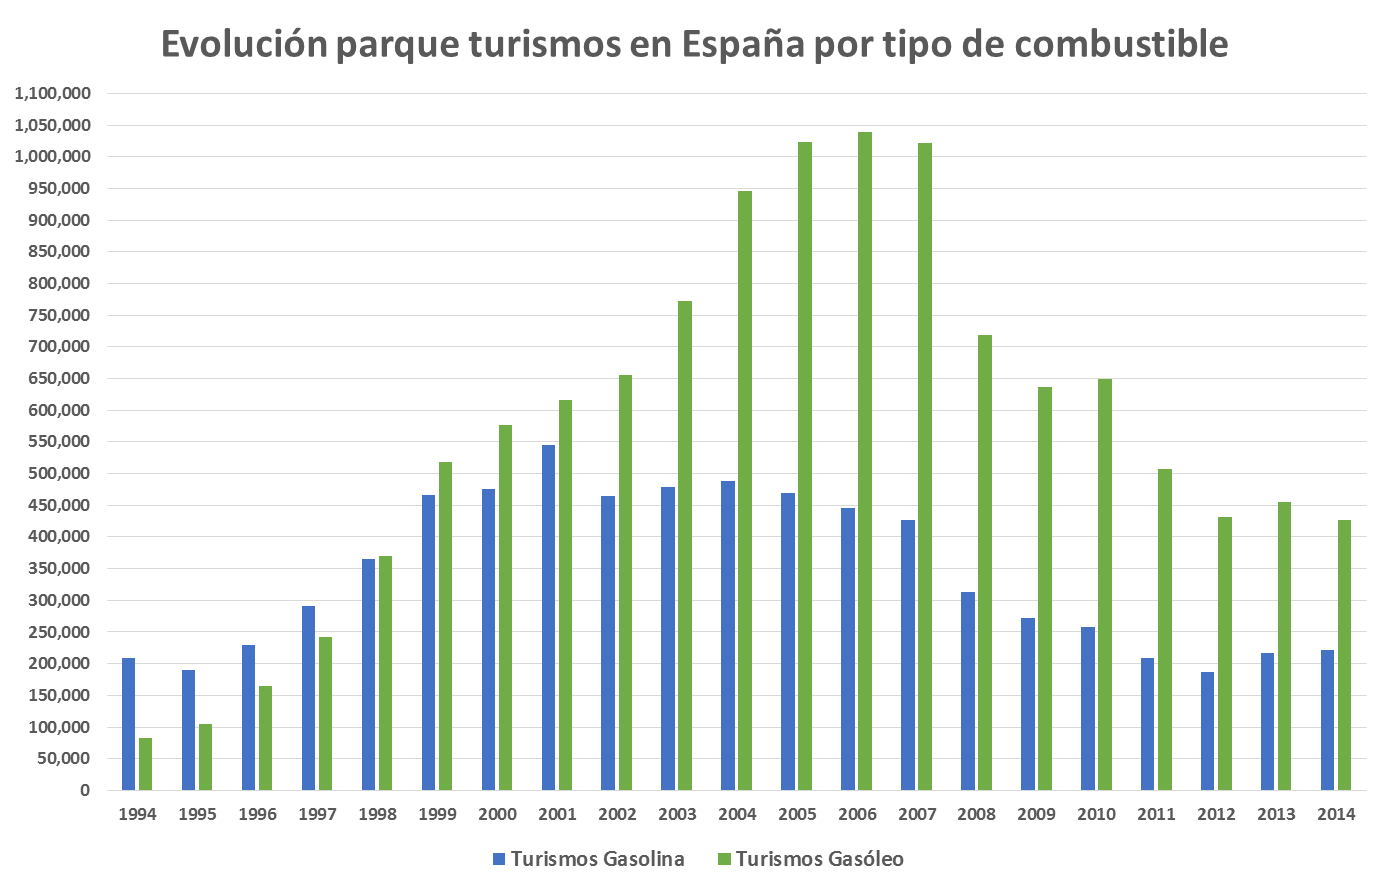
\includegraphics[width=0.6\textwidth]{Evolucionturismos.png}	 
	\caption[Evolución histórica de turismos diésel y gasolina en España]{Evolución parque turismos en España desde 1984 por motorización.\\ \textbf{Fuente:} \href{https://sedeapl.dgt.gob.es/IEST2/menu.do?path=/vehiculos/parque/&file=inebase&type=pcaxis&L=0&js=1}{Portal estadístico de la DGT}}	
\end{figure} \label{fig:EvolucionParqueTurismos}

\par Actualmente la protección del medio ambiente constituye una prioridad ineludible, particularmente en los países avanzados, aunque se ha extendido a la mayoría del resto de países con el Protocolo de Kyoto (1997) y con las cumbres mundiales de Clima, la última de las cuales se celebró en Nueva York (2014). Esta protección del medio ambiente se ha implementado mediante políticas ambientales que cada vez hacen las legislaciones más estrictas. En Europa actualmente están vigentes la Directiva 98/69/CE y la Directiva 2002/80/CE. En estas Normativas se establecen los valores límites para los motores de encendido por compresión ligeros. De las restricciones para los pesados se encarga la Directiva 2001/27/CE. Todas estas directivas establecen límites en términos de masa de partículas emitidas por kilómetro o por kWh.

\par Debido a esto, la mayoría de los estudios sobre emisiones de \index{partículas} partículas analizan exclusivamente los resultados de emisiones en masa. Sin embargo, también la \index{morfología} morfología de las partículas tiene gran importancia dada la notable influencia que ésta tiene sobre la salud humana y sobre el medio ambiente. Por tanto, además de regularse la masa de partículas emitida podría justificarse también algún tipo de regulación sobre el tamaño y la morfología de éstas. En concreto, la legislación medioambiental no es ajena a las normativas sobre el tamaño de las partículas y no es aventurado esperar que en el futuro alguna limitación del tamaño de las partículas se aplique también a las emisiones diésel. Más lejano aún y complejo resulta suponer, de momento, que otros aspectos de la morfología de las partículas puedan llegar a regularse.

\par Por otra parte, antes de ser expulsadas a la atmósfera, la morfología de las partículas tiene también un importante efecto sobre la eficiencia de retención de las \index{trampas de partículas} trampas de partículas, consideradas actualmente como uno de los sistemas de postratamiento necesarios en algunas estrategias de reducción de emisiones más interesantes de cara a cumplir las normativas de emisiones de los motores diésel.

\par Son precisamente los importantes efectos sobre la morfología de las partículas emitidas sobre los filtros de partículas, sobre la salud humana, sobre el medio ambiente y sobre el clima, los que justifican la realización de esta Tesis Doctoral, en línea con el creciente interés científico, como se demuestra en el estudio bibliométrico presentado en el apartado \ref{sec:Bibliometria}.

\section{Objetivos}\label{sec:Objetivos}

\par Principalmente, esta Tesis Doctoral se centra en tres objetivos, que son:

\begin{itemize}
	
	\item Estudio de cómo afecta la no esfericidad de la morfología de las partículas primarias a las características geométricas de los aglomerados diésel. En casi la totalidad de la literatura existente, se parte de la base de que los aglomerados están compuestos por partículas esféricas. Los efectos que pueden llevar a que las partículas no sean perfectamente esféricos son variados y pueden modelarse mediante un parámetro geométrico que permita determinar en qué cuantía la desviación de la idealidad esférica modifica los valores de la geometría fractal. Existen trabajos donde se han modelado estas geometrías, pero la manera en que afectan al prefactor y a la dimensión fractal está menos estudiado. Estos parámetros serán definidos en el capítulo \ref{cap:MetodosAnalisisFractal}. Partiendo de figuras que permiten imponer condiciones de contorno conocidas para dichos parámetros, es posible estudiar cómo se comportan éstos cuando la geometría de las partículas primarias se desvía de la esfericidad.
	
	\item Como se ha comentado anteriormente, para estudiar la geometría fractal de los aglomerados se han de asumir una serie de hipótesis que son aceptadas ampliamente en el ámbito de las emisiones de partículas diésel. Sin embargo, existen muy pocas referencias que cuestionen la validez de dichas hipótesis, o al menos, el rango de valores para los cuales su aplicabilidad está fuera de duda. Esta Tesis tiene como objetivo cuestionar algunas de estas hipótesis, entre ellas la hipótesis del número mínimo de partículas primarias para el cual un aglomerado puede ser considerado fractal o cuasi-fractal.
	
	\item Los fractales, como se expondrá a lo largo del Capítulo \ref{cap:MetodosAnalisisFractal} se encuentran en la naturaleza y es el lenguaje geométrico natural. Parece lógico que una metodología de análisis fractal aplicada al campo de emisiones pueda usarse sin muchas modificaciones a otros campos. Como ejemplo de ello, se aplicarán algunas técnicas a la caracterización fractal de rocas y fracturas hidráulicas usadas para la explotación de hidrocarburos.
	
	\item Con objeto de poder analizar una gran cantidad de parámetros y de morfologías para su posterior comparación, es necesario disponer de herramientas informáticas flexibles y desarrolladas \textit{ad hoc} para las aplicaciones objeto de interés de esta Tesis. Por ello, otro objetivo, aunque menor, de esta Tesis es la mejora y desarrollo de aplicaciones donde se implementen las metodologías desarrolladas en esta Tesis.
	
\end{itemize}

\par Para la consecución del primer objetivo se ha partido del enfoque geométrico seguido en la Tesis de Francisco Martos \cite{martosphD:2006} y en \cite{lapuertaetal:2006,lapuertaetal:2010}. A través de figuras geométricas cuya dimensión fractal es impuesta se pueden determinar el modelo matemático que siguen los parámetros a estudio y ver la influencia de la hipótesis de no esfericidad en la morfología de las partículas diésel. Para un estudio más pormenorizado se utilizó la herramienta informática que de desarrolló en el Proyecto Fin de Carrera \cite{vieraPFC:2014}. El uso de herramientas informáticas es de vital importancia para el estudio de la geometría de aglomerados bajo ciertas condiciones.

\par De igual modo, mediante el uso de otra herramienta informática \cite{delblancoPFC:2015} se puede analizar la dependencia de los resultados con respecto a una de las hipótesis impuestas en los modelos geométricos. Los aglomerados de partículas diésel son asimilados a figuras fractales cuando el número de partículas primarias es superior a cierto número, habiendo un consenso establecido para dicho número, pero sin una justificación lo suficientemente elaborada. La validez en el campo de las partículas diésel, donde los aglomerados tienen usualmente menos de doscientas ($n_{po}\,<\,200$) fue demostrado por \cite{megaridisetal:1990}. Después ha sido utilizado por numerosos autores para la caracterización de hollín \cite{zhuetal:2003,leeetal:2002,caietal:1995,gorbunovetal:1999,zuritaetal:2002,parketal:2004}.

\par El disponer de una metodología que sólo depende de la geometría y no del proceso que da origen a esa morfología, permite que las técnicas y herramientas desarrolladas en la presente Tesis puedan aplicarse a cualquier campo donde la naturaleza fractal de los fenómenos sea relevante.

\section{Antecedentes}\label{sec:Antecedentes}

\par El Grupo de Combustibles y Motores lleva estudiando las emisiones de los Motores diésel durante más de veinte años. Sus esfuerzos se han centrado en la caracterización de combustibles, tanto convencionales como alternativos. Cuando aún la tecnología de motores de encendido por compresión no había superado a la tecnología de los motores de encendido provocado, aunque estaba cerca de lograr este último hito, se presentó la Tesis de Rosario Ballesteros Yáñez \cite{chariphD:2002}. El trabajo de investigación que se presenta en su Tesis Doctoral se enmarca dentro del desarrollo y puesta a punto de herramientas de caracterización y análisis de partículas diésel. Además, los resultados experimentales obtenidos de ensayar combustibles de diferente origen y especificaciones permitieron mejorar el conocimiento que se poseía de los procesos que tienen lugar en el motor y que contribuyen a la generación y emisión de partículas diésel y ayudaron a establecer las directrices en cuanto a búsquedas de posibles nuevos combustibles de automoción y de soluciones óptimas en las que las prestaciones y las emisiones de los motores permaneciesen dentro de unos niveles adecuados. Este trabajo fue el primer estudio que se realizó sobre combustibles y emisiones de partículas diésel dentro de este grupo de investigación y constituyó un antecedente directo de otras Tesis Doctorales. 

\par Tal fue el caso de la Tesis de Francisco Javier Martos Ramos \cite{martosphD:2006}. Fue el primer trabajo dirigido hacia la caracterización morfológica de partículas mediante técnicas fractales. Se propone un método teórico-experimental para determinar los parámetros característicos, desde el punto de vista de la geometría fractal, de las emisiones provenientes de los motores diésel. Como continuación a esta Tesis Doctoral, José Martín Herreros Arellano \cite{martinphD:2009} centró su Tesis en estudiar el efecto del modo de funcionamiento y del combustible en la morfología de las partículas diésel. A partir de micrografías donde se estimaban el radio de giro y él área proyectada, se determinaban parámetros morfológicos de las partículas. Desde el punto de vista de emisiones, existen diferentes estrategias en cuanto a carga y regeneración de trampas de partículas. En este contexto, la Tesis de Fermín Olivas Miñana \cite{ferminphD:2012} se centró en caracterizar la influencia del combustible y de distintas condiciones operativas sobre el tamaño de las partículas, ampliando el estudio presentado en el artículo \cite{lapuertaetal:2007}.

\par Adicionalmente a estas Tesis, cabe mencionar el Proyecto Final de Carrera de Enrique Viera Luis \cite{vieraPFC:2014} que consistió en la implementación de una herramienta informática incluyendo el modelo propuesto en la Tesis de Francisco Javier Martos Ramos \cite{martosphD:2006}, ampliado en los artículos \cite{lapuertaetal:2010} y complementados por el Proyecto Final de Máster de Juan José Expósito González \cite{expositoPFM:2012}, corrigiendo algunas erratas en las ecuaciones de éste último. 

\par Los modelos empleados tienen hipótesis subyacentes que necesitan de herramientas matemáticas para su validación o para la limitación del rango de validez. En este sentido, el Trabajo Final de Grado de Marcos del Blanco Adán \cite{delblancoPFC:2015} desarrolla una metodología computacional ampliamente reconocida y aceptada en el campo de la geometría fractal.
\par El encuadre de la presente Tesis con referencia a los trabajos citados anteriomente se pueden ver en la Tabla.

\section{Metodología}\label{sec:Metodologia}

\par La metodología seguida en esta Tesis tiene un carácter eminentemente teórico. A partir de planteamientos matemáticos no excesivamente complejos se pretende ahondar en el conocimiento de aspectos morfológicos de agregados. Sin embargo, debido a que de abordan temas reales, no se descuida la aplicabilidad práctica de los resultados obtenidos. De igual forma se intentar maximizar las sinergias entre la práctica con la teoría, mediante las bases de datos de imágenes acumuladas desde hace años en el Grupo de Combustibles y Motores de la Universidad de Castilla-La Mancha.

\par La mayor parte de los ensayos se llevaron a cabo en las instalaciones de motores existentes en las Universidades de Castilla-La Mancha y de Málaga. Por un lado, en las primeras hay preparados para diferentes ensayos motores típicos de automoción de inyección directa completamente instrumentados con el triple objetivo de realizar medidas precisas, mantener el control de la instalación y asegurar la repetitividad de las condiciones de ensayo. En etas instalaciones experimentales hay disponibles técnicas experimentales de cierta complejidad que permiten la validación en tendencias de algunos resultados de los modelos planteados, así como otras técnicas experimentales menos complejas cuyos resultados alimentan a los modelos propuestos. Por otro lado, en las últimas hay disponibles técnicas experimentales correspondientes a la visualización de las partículas diésel y su posterior tratamiento digital. Los resultados de estas técnicas son de tipo geométrico y sus resultados son fundamentales para la entrada al modelo planteado sobre la morfología de partículas.

\par Con anterioridad e independencia a esta Tesis se obtuvieron una gran multitud de imágenes de aglomerados. Mediante técnicas de tratamiento de imágenes se pueden tratar para obtener parámetros geométricos característicos y usarlos para alimentar los modelos matemáticos de obtención de propiedades geométricas. Las interconexiones entre los métodos experimentales y teóricos se han esquematizado en la Figura.

\par La incorporación de técnicas de análisis de imágenes de tipo fractal ha permitido calcular la dimensión fractal de aglomerados de geometría conocida. Tal es el caso del método de Box-Counting que se explicará detalladamente en el Capítulo \ref{cap:MetodosAnalisisFractal}. Éste, junto con el resto de técnicas propuestas componen el conjunto de herramientas informáticas utilizadas.

\section{Bibliometría}\label{sec:Bibliometria}

\par Con el fin de demostrar la actualidad del interés de esta Tesis, se han realizado dos estudios bibliométricos, que se detallan en las Figuras y . Estos estudios bibliométricos se han realizado con el \emph{ISI Web of Knowledge} que tiene en su base de datos todas las publicaciones de interés internacional desde 1945.

\section{Viabilidad}\label{sec:Viabilidad}

\section{Desarrollo del Documento de la Tesis}\label{sec:DesarrolloDocumento}

\par La memoria de la presente Tesis Doctoral se compone de un total de nueve capítulos. En el primero de ellos se introduce y se justifica el porqué de la realización de este documento. Se hace una breve descripción de la historia y situación actual del grupo de investigación y se encuadra la Tesis Doctoral dentro de la línea de investigación. Igualmente, se expone la metodología seguida para la realización de la Tesis.

\par El segundo contiene una revisión del estado del arte en la morfología de las partículas en general, y específicamente sobre las partículas diésel. Inicialmente se hace una pequeña revisión a los distintos fenómenos de transporte a los que se pueden ver sometidas las partículas diésel, y que pueden dar lugar a distintos tipos de uniones. Una vez analizado cómo se conforman las partículas diésel desde su nucleación se comentan las distintas maneras de definir el tamaño de éstas y las funciones de distribución típicas. Posteriormente se describen los parámetros utilizados para definir las características morfológicas de las partículas. Se sigue con una descripción de geometrías fractales de campos distintos al de emisión de partículas en procesos de combustión. Finalmente, se comentan las implicaciones de la morfología y el tamaño de las partículas diésel sobre el medio ambiente y sobre la salud pública.

\par Dada la creciente importancia de los fractales en diversas aplicaciones, el capítulo tercero se centra en los métodos de análisis fractal desde un punto de vista puramente teórico. Se dan ejemplos de fractales conocidos y se hace un recorrido por esta incipiente rama de las matemáticas moderna, con reseñas históricas sobre sus principales contribuyentes. De carácter eminentemente teórico, es el capítulo más general de esta Tesis, aunque incluye aplicaciones a diversas ramas de la ingeniería. Una de ellas, las partículas diésel ocupa un apartado dentro de este capítulo. Se sigue con una descripción de otros fenómenos caracterizados por la geometría fractal, como son la caracterización de rocas y de dinámica de fluidos en medios porosos. Finalmente, se tocan otros temas adyacentes y que pretenden despertar la curiosidad de la aplicabilidad de las técnicas fractales como son el análisis de mercados y otras ramas del saber.

\par El cuarto capítulo es una particularización del tercero, centrándose en las partículas diésel. Se comienza dando unos conceptos básicos sobre los métodos geométricos de caracterización de partículas diésel mediante geometría fractal. Estos métodos se centran en la situación ideal de contacto puntual entre partículas. Posteriormente se describe el modelo empleado, desarrollando las ecuaciones matemáticas para los casos estudiados.

\par El quinto capítulo parte del modelo desarrollado en el capítulo anterior, relajando una de las hipótesis empleadas hasta ese capítulo. Se parte de partículas no esféricas, sino que están aplastadas. Primero se describen los procesos por los cuales la geometría de una partícula primaria podría no ser esférica. Después se define el parámetro físico para modelar esta geometría. Por último, se desarrollan las ecuaciones correspondientes y se compara con los resultados obtenidos en el capítulo cuarto.

\par En el sexto capítulo se realiza una crítica de las hipótesis del modelo. Se pretende comprobar la robustez de dichas hipótesis empleando diferentes herramientas matemáticas. Primero se introduce el método del Box-Counting que no depende de la geometría subyacente al problema. Se describe en qué consiste dicho modelo en primer lugar. Después, se aplica a figuras conocidas. Esto es necesario para comprobar la validez de este método. Dos hipótesis se ponen a prueba: la primera, la monodispersidad, es decir, la uniformidad en el tamaño de las partículas primarias que componen el aglomerado. La segunda y última, la esfericidad.

\par Como se ha comentado anteriormente, se dispone de una amplia base de datos con imágenes de aglomerados obtenidos en motores diésel, bien con combustible convencional o biocombustibles. Utilizando las herramientas presentadas en los capítulos anteriores, se pretende caracterizar la "huella" fractal de cada combustible. Para ello, los parámetros geométricos característicos juegan un papel determinante, como se verá en el Capítulo \ref{cap:AplicacionModelo}.

\par La Tesis termina con las conclusiones que se extraen a partir del trabajo realizado y sugerencias de trabajos futuros que se puedan derivar de lo desarrollado en esta Tesis.

\section{Resumen del Capítulo}\label{sec:ResumenCapitulo1}

\newpage
\bibliographystyle{Config/ealpha}	
\bibliography{Chapters/Bibliografia}
		\pagestyle{plain}
\chapter{PROCESOS DE FORMACIÓN \\ Y MORFOLOGÍA DE LAS PARTÍCULAS DIÉSEL} \label{cap:ProcesosFormacionyMorfologia}
\vspace{0.2cm}
\rule{\linewidth}{1.5pt}\\
\startcontents[chapters]
\printcontents[chapters]{}{1}{}
\vspace{0.2cm}
\rule{\linewidth}{1.5pt}\\
%\minitoc
\newpage
\section{Introducción} \label{sec:Introduccion}

\par Durante el proceso de combustión que tiene lugar dentro de la cámara de combustión de un motor diésel el carbono y el hidrógeno que constituyen el combustible se oxidan produciendo luz, dióxido de carbono y vapor de agua. Estos procesos de combustión en motores de combustión interna alternativos permiten al ser humano obtener muchos de los producto y servicios que resultan imprescindibles en la actual sociedad del bienestar. Sin embargo, todo proceso de combustión lleva aparejado un problema de contaminación ambiental. Esto se debe a que la propia composición del combustible, la fluidodinámica de la mezcla aire-combustible y las temperaturas locales dentro de la cámara de combustión hacen que se formen compuestos como el \index{monóxido de carbono}monóxido de carbono, dióxido y trióxido de azufre, compuestos oxigenados de nitrógeno, hidrocarburos y partículas de \index{hollín} hollín. 
\par Las partículas de hollín ha sido objeto de estudio en muchos trabajos, véase por ejemplo \cite{chariphD:2002} u otros muchos autores. La inmensa mayoría de ellos basan sus argumentaciones sobre las emisiones de partículas en los procesos de formación de éstas en el interior de la cámara de combustión. Existen otros tantos autores que estudian el comportamiento y los efectos de las partículas fuera del vehículo, cuando llegan a la atmósfera, como por ejemplo \cite{kimetal:2001} y \cite{siegmannetal:1999}. La razón por la que predominan estos estudios es porque tanto en la cámara de combustión como en la atmósfera, la actividad química es muy importante, a pesar de que en la cámara de combustión lo es con cinéticas muy rápidas (tiempos de residencia muy cortos) y en la atmósfera lo es con cinéticas muy lentas (tiempos de residencia muy largos). Por esto mismo hay pocos autores que estudien la evolución de las partículas a lo largo del tubo de escape. Pero si el aspecto de las partículas que se estudia es el de su morfología, el tránsito de éstas por el tubo no deja a las partículas inalteradas. Por esta razón, esta Tesis Doctoral se centra en el estudio de algunas características morfológicas de las partículas diésel en diversos puntos de escape, si bien nuevamente es necesario recurrir a los procesos de formación en la cámara para explicar muchas de las observaciones.

\par Las características morfológicas en las que se centra esta Tesis son el tamaño y la irregularidad de las partículas diésel. Este capítulo comienza con un epígrafe donde se exponen los distintos fenómenos de transporte que actúan sobre la partícula condicionando el movimiento de ésta en el seno del gas portador. Posteriormente, se describen los distintos fenómenos de transporte que conducen a la conformación de las partículas de hollín hasta adquirir la forma en que circundan el gas. Primero se estudia la generación y el crecimiento de las partículas primarias, posteriormente se describen las distintas uniones a las que se pueden ver sometidas, y por último se estudia cómo la temperatura puede afectar a la estructura de las partículas. Una vez que se ha analizado cómo se pueden conformar las partículas de hollín, se exponen las distintas definiciones de los diámetros característicos de las partículas y las funciones de distribución que los representan.

\par Por último, se resumen lo distintos efectos que tienen las partículas diésel sobre la salud humana y sobre el medio ambiente. Se definirán distintos parámetros para cuantificar dicho impacto y cómo se miden las emisiones. Este estudio del impacto sobre la salud humana y el medio ambiente justifica la realización de estudios como éste, que tienen como objetivo conocer más y mejor la conformación y morfología de las partículas diésel. Dicho conocimiento permitirá diseñar estrategias más adecuadas para reducir en la medida de lo posible este impacto sobre la salud pública y el medio ambiente.

\section{Movimientos de las partículas diésel}\label{sec:Movimientos}

\par La evolución de la composición de un flujo \index{multicomponente} multicomponente (compuesto de $n$ componentes) está gobernada por la ecuación de \index{conservación de las especies} conservación de las especies. Esta ecuación puede plantearse para cada una de las especies aunque lo habitual es plantear $n-1$ ecuaciones con el fin de mantener como ecuación independiente la de continuidad. En general, la ecuación se escribe:

\begin{equation}
\label{ec:continuidad}
\frac{\partial \rho Y_i}{\partial t}\,=\, \nabla \cdot (\rho \vec{c} Y_i)+ \nabla \cdot (\vec{J_i})\,=\, \dot{w}_i
\end{equation}

siendo \nomenclature{$Y_i$}{Concentración de la especie $i$.} $Y_i$ la concentración de la especie $i$, \nomenclature{$\rho$}{Densidad del fluido.} $\rho$ la densidad del fluido y \nomenclature{$\vec{c}$}{Vector velocidad del fluido.} $\vec{c}$ su vector velocidad. La ecuación expresa que las variaciones de concentración con el tiempo (primer término) pueden ser debidas a procesos convectivos, es decir, asociadas a la velocidad de flujo (segundo término), a procesos difusivos (tercer término) o a la presencia de algún término fuente (segundo miembro). Si se considera que la especie $i$ está muy diluida sobre una especie muy abundante y portadora $j$, la expresión más habitual del término difusivo indica que el transporte másico ocurre en la dirección de las concentraciones decrecientes de las especies (ley de Fick):

\begin{equation}
\label{ec:leydefick}
\vec{J}_i\,=\,-\rho D_{ij} \nabla Y_i
\end{equation}

donde \nomenclature{$D_{ij}$}{Coeficiente de difusión de la especie $i$ en la especie $j$.} $D_{ij}$ es el coeficiente de difusión de la especie $i$ en la $j$. Sin embargo, la expresión más general de este término incluye dos términos más, que tienen en cuenta las contribuciones al transporte másico de los gradientes de temperatura y presión, \cite{landauetal:1987}:

\begin{equation}
\label{ec:leydefickgeneral}
\vec{J}_i\,=\,- \rho D_{ij} \left( \nabla Y_i + Y_i \frac{\alpha_T}{T} \nabla T + Y_i \frac{\alpha_p}{p} \nabla p \right)
\end{equation}

donde \nomenclature{$\alpha_T$}{Coeficiente de difusión térmico.} $\alpha_T$ es el \index{coeficiente de difusión térmico} coeficiente de difusión térmico y \nomenclature{$\alpha_p$}{Coeficiente de barodifusión.} $\alpha_p$ el \index{coeficiente de barodifusión} coeficiente de barodifusión.

\par El primer término en la ecuación \ref{ec:leydefickgeneral} es la contribución de la ley de Fick al transporte difusivo total másico, de tal manera que hay un transporte de masa desde las zonas de mayor concentración a las de menor concentración. El segundo término es la contribución cruzada al transporte de masa causada por un gradiente térmico. Este fenómeno es conocido como \index{efecto Soret} efecto Soret. Y el tercer término consiste en la aportación cruzada al transporte másico difusivo a consecuencia de cambios en presiones locales. Según \cite{landauetal:1987} este término difusivo se debe tener en cuenta sólo cuando existen gradientes de presiones considerables en el fluido, como son los casos en que el flujo es transónico o supersónico. Para flujos subsónicos la difusión cruzada a consecuencia del gradiente de presión no es importante.

\par Según la ecuación \ref{ec:leydefickgeneral} el transporte másico difusivo se ha enunciado para la mezcla de dos fluidos, pero igualmente es aplicable a un fluido que no sea homogéneo en sus fases, \cite{masonetal:1962}. En este caso, los anteriores fenónemos de transporte se denominan, respectivamente, \index{difusión browniana} difusión browniana, \index{termofóresis} termofóresis y \index{barofóresis} barofóresis. Si en el seno del fluido existen nanopartículas en suspensión, la difusión másica del fluido afecta directamente al transporte de estas nanopartículas. En efecto, el transporte másico difusivo del gas debido a la variación de la concentración produce fuerzas no equilibradas en las partículas como consecuencia del intercambio de momento desigual entre las partículas y las moléculas del fluido. Estas fuerzas hacen que las partículas se muevan de regiones de mayor concentración a regiones de menor concentración. Este fenómeno es la difusión browniana.

\par El transporte másico difusivo del gas debido al gradiente térmico crea, igual al caso anterior, un movimiento diferencial de las partículas desde las regiones de mayor temperatura a las de menor temperatura. Este efecto es la termofóresis. La barofóresis sólo es significativa bajo grandes gradientes de presión. Y por último, en el caso de que la mezcla gaseosa portadora de partículas no sea uniforme en composición, las partículas en suspensión están sometidas a una fuerza debida a los gradientes de concentración de los componentes gaseosos. Este fenómeno de transporte másico de partículas se llama \index{difusiofóresis} difusiofóresis, y ha sido despreciado en la ecuación \ref{ec:leydefickgeneral}, ya que se considera que la mezcla gaseosa es uniforme.

\par En el caso particular del flujo de escape de un motor diésel tanto la barofóresis como la difusiofóresis se pueden despreciar frente a la difusión browniana, por las razones apuntadas. Sin embargo, la termofóresis no se puede despreciar ya que los gradientes de temperaturas sí son significativos, sobre todo entre el gas y el tubo de escape, radialmente.

\par El movimiento de las partículas diésel en el seno del gas de escape se debe fundamentalmente a dos fenómenos, al difusivo (difusión browniana y termofóresis) y al arrastre que ejerce el gas sobre la partícula, el cual es asimilable a un movimiento convectivo. Este fenómeno aparece siempre y cuando haya una diferencia de velocidades entre la partícula y el gas. Las partículas con tamaños de unidades o decenas de nanómetros se caracterizan porque sus colisiones son principalmente de carácter browniano, es decir, son provocadas por el movimiento browniano. Esto sucede siempre y cuando la distancia media recorrida entre choques de partículas sea del orden de pocos nanómetros, es decir del propio tamaño de las partículas. También suceden colisiones brownianas cuando la temperatura a la que están las partículas es muy elevada, ya que la distancia media recorrida en el movimiento browniano de las partículas es directamente proporcional a la temperatura de la misma. Las simulaciones realizadas por \cite{frenklach:2002}, \cite{kazakovetal:1998} y \cite{stasioetal:2002} demuestran que las colisiones entre partículas primarias que ocurren en el interior de la cámara de combustión, donde la temperatura es muy alta, son de tipo browniano.

\par \cite{kimetal:2002} y \cite{kimetal2:2002} realizan una simulación para las colisiones de material particulado una vez que llegan al ambiente. \cite{hisaedaetal:2000} y \cite{hayasietal:1999} realizan simulaciones en el interior del tubo de escape en condiciones especiales, es decir, no comunes en el funcionamiento de un motor diésel. En estos casos consideran que las colisiones son del tipo browniano, porque la concentración es muy alta, es decir, la distancia entre partículas es del orden del movimiento de tipo browniano característico de cada partícula.

\par En el caso del flujo en el tubo de escape, la temperatura del gas no es elevada y además la concentración de material particulado tampoco lo es. En estas condiciones las colisiones de las partículas diésel no tienen, en su generalidad, carácter browniano sino que son ocasionadas por el arrastre del fluido sobre las partículas. También, en estas condiciones (condiciones características dentro del tubo de escape) el camino libre medio que tiene que recorrer una partícula para colisionar con otra es de varios órdenes superior a la distancia media recorrida por la partícula en su movimiento de tipo browniano.

\section{Procesos de formación de las partículas}
\subsection{Introducción}

\par Los aglomerados diésel de hollín están compuestos por partículas primarias. Tal y como se explica en \cite{varios:2011} se considera \index{partícula primaria} como partícula primaria a cualquier materia presente en los gases de salida que se encuentre en estado líquido o sólido en condiciones aproximadamente ambientales. La consecuencia directa de esta definición es que a la hora de analizar las emisiones de partículas es imprescindible estudiar el proceso de dilución del escape con el aire ambiente. Las partículas primarias presentan geometrías muy similares a esferas, como se muestra en la Figura \textit{incluir referencia a la figura}. Además, tanto el diámetro medio de estas partículas como la desviación típica del diámetro medio varían muy poco en función de las distintas condiciones de funcionamiento del motor, \cite{leeetal2:2002}, \cite{zhuetal:2003}.  Es usual describir las partículas primarias con una función de distribución de tamaños uniforme, es decir monodispersa, con diámetros medios del orden de 25 nm, \cite{smallwoodetal:2002, wentzeletal:2003}. Aunque dos aglomerados tengan el mismo número de partículas primarias, éstas se disponen en cada aglomerado de manera distinta, haciendo que cada uno tenga una forma irregular distinta, con diferente compactación y tamaño, y por lo tanto con diferente densidad aparente, \cite{lapuertaetal:2003}. Contrariamente a las partículas primarias, los aglomerados no son uniformes ni en tamaño ni en forma. En realidad son polidispersos, así que para su descripción es necesario hacer un estudio estadístico.

\par Como argumenta R. Ballesteros \cite{chariphD:2002} y se encuentra sucintamente expuesto en \cite{varios:2011}, los procesos físicos y químicos que intervienen en la cámara de combustión de las partículas diésel son numerosos y complejos. Debido a que estos procesos físicos y químicos pueden ocurrir tanto en la línea de escape como en el momento de dilución en la atmósfera (Figura \ref{fig:procesosformacionyemision}), se considera que una determinación exacta de las emisiones de partículas requiere una simulación de estos procesos de dilución, procesos que obligan a distinguir entre \index{partículas primarias} partículas primarias, aquellas que se forman directamente como producto de la combustión y se miden justo a la salida del cilindro, y \index{partículas secundarias} partículas secundarias, resultantes de alguno de los procesos atmosféricos mencionados anteriormente, tanto en el escape como ya directamente en la atmósfera, y que se recogen usualmente mediante sistemas de dilución situados al final del sistema de escape o en una derivación del mismo. Son precisamente estas partículas secundarias aquellas que son limitadas en las diferentes normativas mundiales.

\begin{figure}[ht]
\centering
	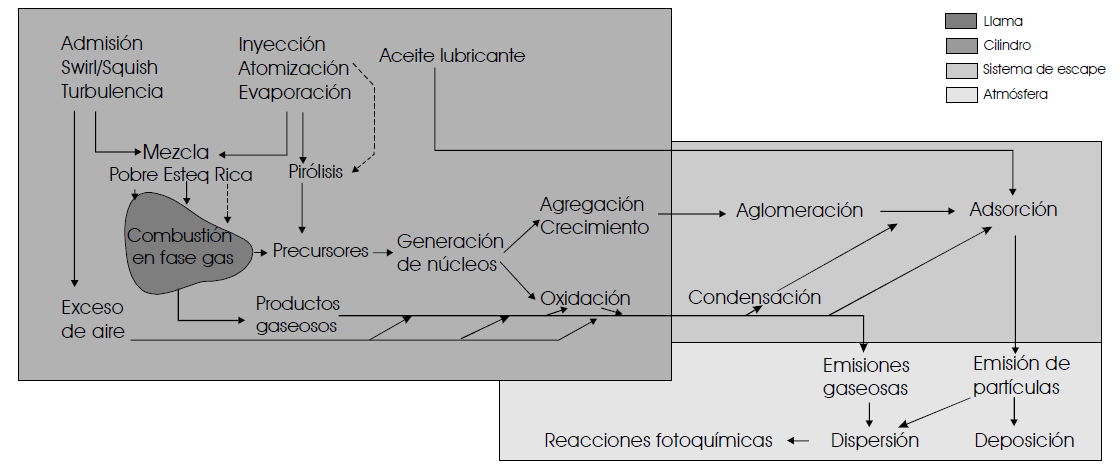
\includegraphics[width=0.9\textwidth]{EsquemaformacionyEmision.png}	 
	\caption{Esquema de formación y emisión de partículas} \label{fig:procesosformacionyemision}
\end{figure} 

\par En este apartado, se describirán las características físicas y químicas de las partículas partiendo del estudio del substrato inicial (hollín), sus principales mecanismos de formación, así como su composición y sus características morfológicas:

\begin{enumerate}
\item Hollín.
\item Formación de las partículas y composición.
\item Distribución de tamaños de partículas
\end{enumerate}

\subsubsection{Hollín}

\par Existe un límite teórico para la aparición de partículas de hollín que se puede calcular planteando la siguiente reacción para un combustible genérico oxigenado:

\begin{equation}
\label{ec:limitehollin}
C_nH_mO_p + yO_2 \rightarrow (p + 2y)CO + \left( \frac{m}{2} \right) H_2 + (n-p-2y)C_{(s)}
\end{equation}

Según la reacción \ref{ec:limitehollin}, planteada inicialmente para combustibles convencionales \cite{haynessetal:1981}, el límite de \index{dosado} dosado local que favorece la aparición de hollín se calcula para $n\,=\,2p+y$. En esas condiciones la relación masa de combustible frente a masa de agente oxidante es igual al:

\begin{equation}
\label{ec:relacionmasacombagoxidantedosadofavorecehollin}
\frac{m_f}{m_{O_2}}\,=\,\dfrac{12n+m+16p}{(n-p)16}\,=\,\dfrac{0,75+0,0625\frac{m}{n}+\frac{p}{n}}{1-\frac{p}{n}}
\end{equation}

\par Si se plantea la reacción estequiométrica \ref{ec:hollinestequiometrico}:

\begin{equation}
\label{ec:hollinestequiometrico}
C_nH_mO_p + \left( n + \frac{m}{4} - \frac{p}{2} \right) O_2 \rightarrow nCO_2 + \left( \frac{m}{2} \right) H_2O
\end{equation}

\par La relación entre la masa de combustible y la masa de agente oxidante para esta reacción es:

\begin{equation}
\label{ec:relacionmasacombagoxidanteestequiometrico}
\left( \dfrac{m_f}{m_{O_2}} \right)_e\,=\,\dfrac{12n+m+16p}{\left( n + \frac{m}{4} - \frac{p}{2} \right)32}\,=\,\dfrac{0.375+\frac{m}{n}+0.5\frac{p}{n}}{1+0.25\frac{m}{n} - 0.5\frac{p}{n}}
\end{equation}

\par Teniendo en cuenta las expresiones \ref{ec:relacionmasacombagoxidantedosadofavorecehollin} y \ref{ec:relacionmasacombagoxidanteestequiometrico} se puede calcular el dosado relativo que se plantea como límite teórico para la aparición de hollín como:

\begin{equation}
\label{ec:dosadorelativoaparicionhollin}
F_r\,=\, \dfrac{2+0.5\frac{m}{n}-\frac{p}{n}}{1-\frac{p}{n}}
\end{equation}

La figura \ref{fig:limiteteoricoaparicionhollin} representa este límite teórico en función de la relación $m/n$ y $p/n$ del combustible. Si se asume, de acuerdo con el modelo de Dec, que una de la principales fuentes de formación de hollín en motores diésel es la región de combustión premezclada rica que tiene lugar tras el \textit{lift off}, cuyo dosado relativo se encuentra alrededor de 4 \cite{lapuertaetal:2010}, se puede comprobar que existen algunos combustibles con altos valores de $m/n$ y $p/n$ (estos últimos combustibles oxigenados) cuyos valores de dosado relativo límite de formación de hollín es claramente superior.

\begin{figure}[ht]
\centering
	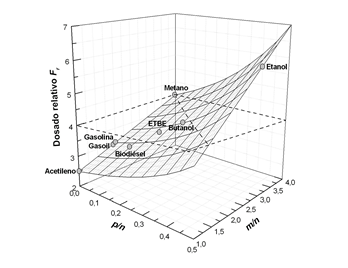
\includegraphics[width=0.6\textwidth]{LimiteTeoricoAparicionHollin.png}	 
	\caption{Límite teórico de aparición de hollín} \label{fig:limiteteoricoaparicionhollin}
\end{figure} 

\par Los mecanismos que envuelven el proceso de generación de partículas de hollín han sido extensamente estudiados. En general, los investigadores coinciden en la mayor probabilidad de colisión de dos compuestos aromáticos policíclicos, que conduce a asumir que la primera partícula carbonosa o núcleo de hollín que se forma se produce tras esta colisión, dando lugar a una partícula tridimensional. Otra de las vías de formación de núcleos de hollín pasa por reacciones de deshidrogenación de moléculas del combustible bajo temperaturas locales muy elevadas sin pasar por la formación de especies aromáticas precursoras. La formación de hollín en motores diésel por esta ruta no es predominante debido a las temperaturas características del proceso de combustión en estos motores (Figura \ref{fig:esquemaprocesoformacionhollin}).

\begin{figure}[ht]
\centering
	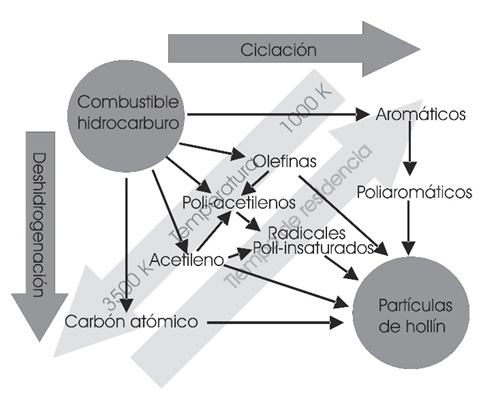
\includegraphics[width=0.6\textwidth]{Esquemaprocesodeformaciondehollin.png}	 
	\caption{Esquema de los procesos de formación de hollín} \label{fig:esquemaprocesoformacionhollin}
\end{figure} 

\par El hollín formado se compone de partículas carbonosas (partículas primarias) estructura-das en redes cristalinas que contienen alrededor de un 1 \% en peso de hidrógeno, es decir, la proporción correspondiente a la fórmula empírica media de $C_8H$ (Figura \ref{fig:esquemaformacionparticulasprimariashollin}). Cada átomo de hidrógeno, que se separa durante la deshidrogenación, activa a otra molécula produciendo su nucleación y crecimiento, adoptando estructuras en forma de red. Este proceso tiene lugar principalmente en la superficie de llamas poco expuestas al oxígeno del aire en un rango estrecho de altas temperaturas. La microestructura de las partículas primarias es similar a la del grafito, en la que la red cristalina está formada por estructuras hexagonales denominadas láminas de grafeno. Estas láminas de grafeno se unen formando cristales (típicamente se encuentran alrededor de 2 a 5 láminas por cristal), que a su vez se unen con diferentes orientaciones formando las partículas primarias de hollín (del orden de $10^3-10^4$ cristales y $10^5-10^6$ átomos de carbono por partícula primaria). 

\begin{figure}[ht]
\centering
	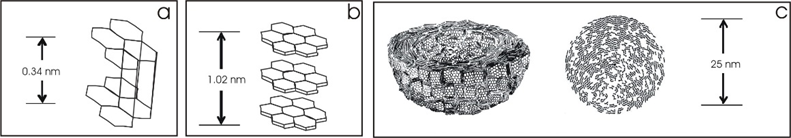
\includegraphics[width=\textwidth]{Esquemaformacionparticulasprimariashollin.png}	 
	\caption[Esquema de formación de partículas primarias de hollín]{Esquema de formación de partículas primarias de hollín: (a) láminas de grafeno (b) cristales y (c) partículas primarias} \label{fig:esquemaformacionparticulasprimariashollin}
\end{figure} 

A continuación se describe brevemente cada una de las etapas que conducen a la forma-ción de partículas de hollín desde la llama al sistema de escape (Figura \ref{fig:procesosformacionyemision}): 

\begin{enumerate}
\item Formación de especies precursoras.
\item Generación o nucleación de partículas de hollín (partículas primarias).
\item Oxidación de las partículas.
\item Crecimiento de la superficie de las partículas y aglomeración de las mismas.
\item Condensación y/o adsorción de hidrocarburos en la superficie de las partículas.
\end{enumerate}

\par Por la válvula de escape pueden salir partículas primarias de hollín además de aglomerados de partículas primarias de hollín (partículas secundarias).

\subsubsection{Nucleación de las partículas}\label{subsubsec:nucleacion}

\par es el proceso en el que se produce la formación de una fase sólida (partículas de hollín) desde una fase vapor en regiones localmente ricas de combustible y alta temperatura (entre 1300-1600 K). Este proceso, generalmente, consiste en la adición de pequeños hidrocarburos radicales (acetileno y otros precursores en fase gas) a moléculas aromáticas de mayor tamaño, hasta que éstas alcanzan un tamaño suficiente como para convertirse en un núcleo de partícula con un diámetro en el rango de 1-2 nm y 10 uma (unidades de ma-sa atómica). Este núcleo posteriormente en la etapa de crecimiento superficial irá progresivamente disminuyendo su proporción de hidrógeno. Debido a su pequeño tamaño estas partículas no contribuyen significativamente a la masa total de hollín, pero sí tienen una influencia muy significativa en la producción final de hollín, ya que actúan como núcleos para el posterior crecimiento superficial. La nucleación tiene lugar cerca de la zona de reacción primaria donde la temperatura y la concentración de radicales e iones son máximas, tanto en llamas premezcladas como en difusivas. 

\subsubsection{Crecimiento superficial de las partículas}\label{subsubsec:crecimientosuperficial}

\par El crecimiento de la partícula puede deberse al propio crecimiento superficial de la partícula, a la coagulación entre partículas, a la agregación o a la aglomeración. El crecimiento de la partícula por coagulación, agregación y aglomeración, se trata en los epígrafes posteriores.

\begin{enumerate}
\item Superficial: en esta etapa se produce la adición de masa en la superficie de una partícula ya nucleada. En este proceso se añaden hidrocarburos en fase gas, generalmente acetilenos e HAP, en los sitios reactivos de la superficie de las partículas y a alta temperatura. Esta etapa suele ocurrir simultáneamente a la nucleación, no pudiéndose distinguir entre el final de la nucleación y el comienzo del crecimiento superficial. Aquí es donde se produce la mayor parte de la masa de hollín, por tanto es importante el tiempo que se encuentran las partículas en esta etapa para determinar la cantidad másica y volumétrica de hollín, mientras que el número de partículas no se ve afectado por este proceso. El crecimiento superficial continúa desde la zona de reacción primaria hasta otras regiones con una menor temperatura y menor concentración de hidrocarburos. La tasa de crecimiento superficial de las partículas de menor tamaño es más alta que las de mayor debido a que tienen más sitios activos (con radicales activos) por unidad de masa \cite{hiroyasuetal:1976}.  

\item Coagulación: es un fenómeno físico, no químico. La coagulación o coalescencia se produce por colisión de dos partículas primarias aproximadamente esféricas, obteniéndose una única partícula resultante manteniendo la identidad esférica y cuya masa es la suma de las masas de las dos partículas primarias que intervienen en la colisión. Por tanto, este proceso resulta en una reducción significativa del número de partículas, un aumento del tamaño de las mismas manteniendo constante la masa de las partículas \cite{haynessetal:1981}. 
\end{enumerate}

\subsubsection{Oxidación}\label{subsubsec:oxidacion}

\par La oxidación es el proceso mediante el cual se produce la conversión de carbono o hidrocarburos a productos de la combustión, que generalmente son $CO$ (oxidación parcial), $CO_2$ (oxidación completa) y agua. Aunque el oxidante inicialmente es el oxígeno del gas admitido, otros productos de la disociación de éste (como el oxígeno atómico) y de las primeras etapas de la combustión (el radical hidroxilo OH) actúan como oxidantes de los propios productos intermedios generados y en particular del hollín formado. La oxidación por el radical OH es predominante bajo condiciones ricas y estequiométricas del combustible, mientras que en condiciones localmente pobres (alto dosado) participan tanto el radical hidroxilo como el oxígeno molecular. El proceso de oxidación a $CO$ y $CO_2$ tanto de los HAP como del hollín es un proceso que compite con el de formación y como resultado de estos dos procesos contrapuestos se obtiene su tasa neta de formación. El proceso de oxidación del carbono perteneciente a una partícula de hollín se produce en dos etapas. En la primera etapa se produce la adsorción del oxidante a la superficie de la partícula y en la segunda se produce la desorción del producto oxigenado ($CO$ ó $CO_2$) desde la superficie de la partícula. El proceso de oxidación comienza a temperaturas superiores a 1300 K debido a la microestructura tipo grafítica que dota de una gran resistencia a la oxidación de las partículas. El modelo más usado respecto de la oxidación es el modelo semiempírico de Nagle y Strickland-Constable que correlaciona la oxidación de pirografito para presiones parciales de oxígeno entre 0.1 y 0.6 atmósferas y un rango de temperaturas de 1100-2500 K. En general, se puede afirmar que la velocidad de oxidación se incrementa hasta los 2000 K, siendo a partir de este punto cuando la velocidad de oxidación permanece prácticamente constante, como puede observarse en la Figura \ref{fig:velocidadoxidacionhollinllamas}.

\begin{figure}[ht]
\centering
	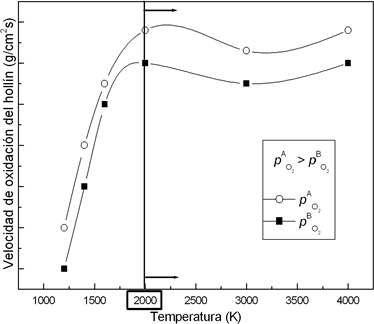
\includegraphics[width=0.5\textwidth]{VelocidadOxidacionHollinLlamas.png}	 
	\caption{Velocidad de oxidación del hollín en llamas} \label{fig:velocidadoxidacionhollinllamas}
\end{figure} 

\subsubsection{Aglomeración y agregación}\label{subsub:aglomeracionyagregacion}

\par Estos dos conceptos son ligeramente diferentes, la agregación es la unión de partículas mediante fuerzas cohesivas atómicas o moleculares produciendo agregados lineales de gran estabilidad. Y la aglomeración es la unión mediante fuerzas de cohesión débiles como por ejemplo la tensión superficial. En la mayoría de las situaciones se usan los términos de agregación (agregado) y aglomeración (aglomerado) indistintamente para referirse a la consecuencia de las colisiones entre partículas y/o aglomerados/agregados de partículas (Figura \ref{fig:fototemagregadohollin}). La aglomeración, al igual que la coagulación, supone una considerable disminución del número de partículas/aglomerados y un aumento del tamaño de los aglomerados, mientras que no se modifica la masa de las partículas. Una vez se han formado las partículas primarias, en primer lugar éstas colisionan entre sí formando aglomerados de mayor tamaño compuestos por varias partículas primarias. Pero a continuación, pueden producirse colisiones entre partículas primarias y los aglomerados y colisiones entre los aglomerados. En función de la relación entre el camino libre medio (distancia que recorre una partícula/aglomerado entre colisiones sucesivas) y el tamaño de la partícula/aglomerado existen diferentes tipos de aglomeraciones (en régimen balístico y limitadas por difusión) que tienen como consecuencia la forma del aglomerado, que es cuantificada por medio de su dimensión fractal. 
Algunas de estas estructuras de hollín formadas durante estos procesos son muy estables, pero otras tienen reacciones de formación muy reversibles, y el contacto con radicales hidroxilo a alta temperatura favorece su reconversión a hidrocarburos aromáticos policíclicos.

\begin{figure}[ht]
\centering
	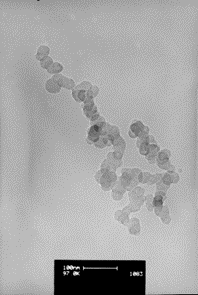
\includegraphics[width=0.3\textwidth]{FotoTEMagregadohollin.png}	 
	\caption[Microfotografía TEM de un agregado de hollín]{Microfotografía TEM de un agregado de hollín recogido por termofóresis y compuesto por partículas primarias} \label{fig:fototemagregadohollin}
\end{figure} 

\par Algunas de estas estructuras de hollín formadas durante estos procesos son muy estables, pero otras tienen reacciones de formación muy reversibles, y el contacto con radicales hidroxilo a alta temperatura favorece su reconversión a hidrocarburos aromáticos policíclicos.

\subsection{Formación de partículas y composición}\label{subsec:formacionparticulasycomposicion}

\par A lo largo del conducto de escape se produce una reducción de temperatura del gas y los agregados/aglomerados de hollín pueden verse sometidos, bajo estas circunstancias, a fenómenos de adsorción y de condensación de hidrocarburos ya sea por condensación superficial o como nucleación de gotas líquidas (Figura \ref{fig:esquemaprocesoformacionhollin}). Sin embargo, estos procesos ocurren mayoritariamente en el proceso de dilución (proceso que define a las partículas) y en función de cómo se realice este proceso y las características del gas de escape, estos fenómenos pueden acentuarse o verse reducidos. 

\par El fenómeno de adsorción consiste en el crecimiento de la partícula por la adhesión en fase gas de moléculas de hidrocarburos sin quemar o parcialmente quemados a la superficie de la partícula de hollín por medio de fuerzas tanto químicas como físicas (fuerzas de Van der Waals). Por otro lado, el crecimiento también puede ser por condensación cuando los hidrocarburos que se añaden a la superficie de las partículas se encuentran en fase líquida. Por último, la nucleación es la formación de un pequeño núcleo a partir de los hidrocarburos en fase líquida. El hecho de que se produzca uno u otro fenómeno depende fundamentalmente del grado de saturación  (cociente entre la presión parcial del hidrocarburo en el gas de escape y la presión de saturación del mismo) y de la superficie de la partícula disponible en el gas de escape. Cuando el grado de saturación es menor que uno el único mecanismo posible de adición de hidrocarburos a las partículas es la adsorción en fase gaseosa, mientras que si es mayor que uno se puede producir adsorción desde fase condensada o nucleación de hidrocarburos. Si no existe superficie disponible para que los hidrocarburos se adsorban o condensen y el grado de saturación es mayor que la unidad, esos hidrocarburos se nuclearían, dando lugar a pequeñas gotas líquidas de hidrocarburos, que generalmente son las responsables de la existencia de una moda denominada moda núcleos (Figura \ref{fig:distribuciontipicaparticulas}) en las distribuciones de tamaños de partículas. 

\begin{figure}[ht]
\centering
	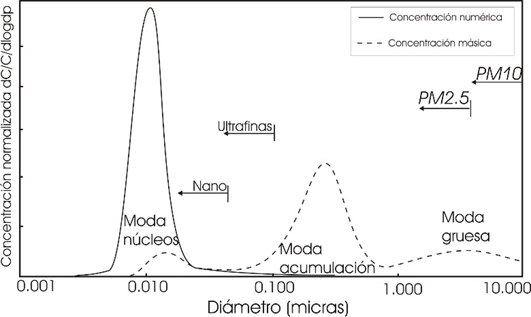
\includegraphics[width=0.8\textwidth]{Distribuciontipicaparticulas.png}	 
	\caption{Distribución típica de los tamaños de partículas} \label{fig:distribuciontipicaparticulas}
\end{figure} 

\par Estos procesos, como ya se ha comentado, pueden ocurrir en el conducto de escape, pero sobre todo, tienen lugar en el proceso de dilución. Por tanto, en función de cómo se haga este proceso se puede llegar a condiciones favorables para que los fenómenos de adsorción y condensación se produzcan o se puedan evitar. En la Figura \ref{fig:esquemaprocesodilucion} se muestra cualitativamente cómo sería el proceso de dilución en función de tres diferentes grados de dilución partiendo del estado inicial denotado como 0. Si el grado de dilución es pequeño el proceso acabaría en el punto 1, el cual está bastante alejado de la curva de saturación del hidrocarburo y por tanto, la probabilidad de producir nucleación es baja. Si se aumenta el grado de dilución a uno intermedio denotado como 2, este punto está bastante más cerca de la zona de saturación siendo máxima la probabilidad de nucleación. Por último, si se aumenta el grado de dilución hasta llegar a 3, la probabilidad de nucleación es menor ya que este punto está más alejado de la zona de saturación que el punto 2. En la misma figura, se puede apreciar el efecto que sobre estos fenómenos tiene también la temperatura del gas de escape. Cuando ésta es mayor (punto 0'), la probabilidad de nucleación es menor puesto que la región de saturación se aleja con respecto al caso de una menor temperatura de escape. 

\begin{figure}[ht]
\centering
	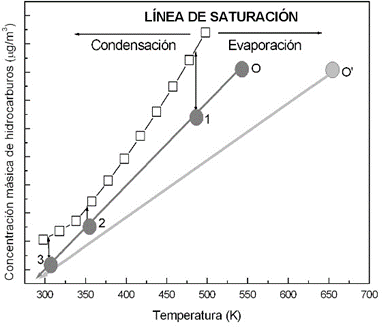
\includegraphics[width=0.8\textwidth]{Esquemaprocesodilucion.png}	 
	\caption{Esquema del proceso de dilución para diferentes grados de dilución y temperaturas} \label{fig:esquemaprocesodilucion}
\end{figure} 

\par Los procesos que conducen a la formación de partículas condicionan su composición \cite{smith:1982}. Las partículas están compuestas por dos fracciones fácilmente separables mediante un proceso de extracción química:

\begin{enumerate}
\item Una fracción insoluble que puede tener compuestos orgánicos e inorgánicos denominada comúnmente ISF, en la que prevalece principalmente el carbono (hollín), acompañado por otros compuestos tales como sulfatos, sales, agua y materiales inorgánicos procedentes de aditivos.
\item Una fracción orgánica soluble (SOF), denominada así por su solubilidad en el disolvente orgánico empleado en la extracción, compuesta por hidrocarburos y otros compuestos orgánicos procedentes directamente del combustible  y del aceite lubricante, o bien de reacciones en el interior de la cámara de combustión en el caso del combustible inyectado. Esta adhesión al substrato de hollín ocurre mediante los procesos de condensación y adsorción que tienen lugar durante su recorrido por el sistema de escape, donde el descenso de temperatura se hace más rápido.
\end{enumerate}

\par Una composición media típica de las partículas emitidas se muestra en la Figura \ref{fig:ejemplocomposiciontipicaparticulas}

\begin{figure}[ht]
\centering
	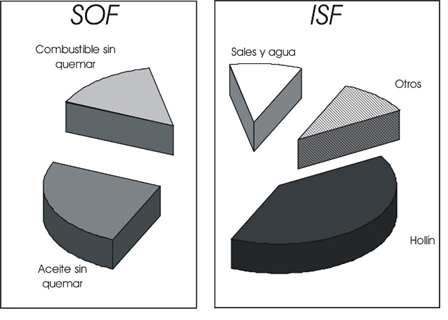
\includegraphics[width=0.6\textwidth]{Ejemplocomposicionquimica.png}	 
	\caption{Ejemplo de composición típica de las partículas} \label{fig:ejemplocomposiciontipicaparticulas}
\end{figure} 

\par Aunque la separación de las partículas diésel en ISF y SOF es la más ampliamente extendida en bibliografía, no es la única. Algunos trabajos utilizan métodos térmicos para separar las partículas en dos fracciones, una volátil denominada VOF y compuesta por hidrocarburos y otros compuestos orgánicos y agua, y otra fracción no volátil, principalmente formada por hollín.

\par En todo caso, e independientemente del método utilizado para determinar la composición de las partículas, los dos principales componentes de éstas son el hollín, presente en la ISF si se emplea extracción química o en la fracción no volátil si se emplean métodos térmicos, y los hidrocarburos y demás compuestos orgánicos, que forman parte de la SOF en el caso de la extracción química o de la VOF en el caso de los métodos térmicos.

\subsection{Colisiones entre partículas} \label{subsec:colisiones}

\par Tras la colisión entre dos partículas puede suceder que éstas se disgreguen en más de dos partículas o que se unan. Que ocurra una u otra cosa depende, fundamentalmente, de la energía cinética de ambas partículas en el momento de la colisión y de las fuerzas coercitivas internas que tenga cada partícula. Por lo general, la colisión entre partículas tiene como consecuencia la unión de las dos partículas que colisionan, las cuales dejan de existir como tales, para formar parte de una partícula nueva cuya masa es la suma de las masas de las partículas y cuya velocidad es aquélla que cumple la conservación de la cantidad de movimiento. Esta descripción de las colisiones es muy simple, pues en realidad en la formación de la partícula nueva intervienen más factores además de la masa de las partículas originales.

\par La colisión se debe a dos fenómenos principalmente. Por un lado la colisión debida a la difusión, básicamente browniana, entre partículas, y por otro lado la colisión debida a acciones forzadas sobre las partículas, tales como la convección del propio fluido, acciones gravitacionales, acciones magnéticas o eléctricas sobre partículas.

\par Cuando colisiona una partícula cualquiera de masa $m_i$ con su complementaria hasta $m$, es decir, con una partícula de masa $m - m_i$, se genera una nueva partícula de masa $m$. La evolución de la función de distribución de masa de partículas debida a las colisiones se modela mediante la siguiente ecuación integro-diferencial, \cite{fuchs:1989}:

\begin{equation}
\label{ec:colisionesintegrodiferencial}
\dfrac{dn(m,t)}{dt}\,=\, \frac{1}{2} \int_0^m K(m_i,m-m_i)n(m_i)n(m-m_i)dm_i-n(m)\int_0^\infty K(m,m_i)n(m_i)dm_i
\end{equation}

donde $m$ es la masa de la partícula formada como consecuencia de la colisión entre dos partículas de masa $m_i$ y $m-m_i$, $n(m_i)$ es el número de partículas con masa $m_i$. $K$ es la frecuencia de colisiones entre dos partículas cualesquiera. La variación temporal del número de partículas con masa $m$ depende de la producción de partículas de masa $m$ y de la pérdida de las partículas de masa $m$ que se hayan generado en un tiempo anterior. El primer sumando de la derecha de la ecuación \ref{ec:colisionesintegrodiferencial} representa la producción de partículas de masa $m$ en el instante actual. A este sumando hay que afectarle del coeficiente 0.5, ya que por cada dos partículas que colisionan se forma una nueva partícula. El segundo sumando de la ecuación \ref{ec:colisionesintegrodiferencial} representa la pérdida de partículas de masa $m$ debida a las colisiones de partículas de masa $m$ con otras para formar partículas mayores. La ecuación \ref{ec:colisionesintegrodiferencial} no es única: en realidad es un sistema de ecuaciones. Además el término integral no es del todo apropiado ya que las partículas son discretas, por lo que habría que utilizar sumatorios \cite{friedlander:2000}.

\begin{equation}
\label{ec:colisionessumatorio}
\dfrac{dn(m_k)}{dt}\,=\, \frac{1}{2} \sum_{\substack{i\,=\,1 \\ j\,=\,1}}^{i+j=k} K(m_i,m_j)n(m_i)n(m_j)-n(m_k)\sum_{i\,=\,1}^{i\,=\, \infty} K(n_m,m_i)n(m_i)
\end{equation}

Si se supone una frecuencia de colisiones constante, $K$, y un aerosol inicial monodisperso $n(t\,=\,0)$, la solución de la ecuación \ref{ec:colisionesintegrodiferencial} se reduce a:

\begin{equation}
\label{ec:solucioncolisiones}
n(t)\,=\, \dfrac{n(t\,=\,0)}{1+n(t\,=\,0)Kt}
\end{equation}

\par Según la ecuación \ref{ec:solucioncolisiones} el número de partículas decrece conforme pasa el tiempo, haciendo que el tamaño de las partículas sea más grande.

\par Para un aerosol polidisperso en el que se suponga que la frecuencia de colisiones sea constante, la ecuación \ref{ec:colisionesintegrodiferencial} tiene solución analítica, \cite{fuchs:1989}. En realidad la frecuencia de colisiones no es constante, sino que depende de la temperatura de las partículas, de la viscosidad dinámica del gas, y de otros muchos factores.

\par Los otros fenómenos que producen colisiones entre partículas se modelan mediante una función de frecuencia de colisiones específica para caso de estudio, \cite{friedlander:2000}. Existen muchos autores que se han dedicado a modelar estas funciones de frecuencia de colisiones, \cite{kazakovetal:1998,kimetal:2001,kostoglouetal:2001}, etc.

\par En cualquier caso, planteamientos como el descrito permiten predecir el crecimiento másico de las partículas, pero no dan información sobre la morfología de las mismas. Para esto, es necesario tener en cuenta que las colisiones pueden tener como consecuencia uniones muy diversas.

\subsection{Tipos de uniones}

\par Simultáneamente al proceso de crecimiento de las partículas primarias, e igualmente una vez terminado éste, las partículas están sometidas a movimientos microscópicos (comentados en el epígrafe \ref{sec:Movimientos}), que tienen como consecuencia frecuentes colisiones entre ellas. Las consecuencias de estas colisiones pueden ser diversas, en función de las condiciones ambientales en las que se encuentran las partículas primarias:

\begin{itemize}

\item Coagulación: dos partículas, por ejemplo esféricas, coagulan si como consecuencia de la colisión entre ellas y a causa de las condiciones ambientales de presión y temperatura elevadas, la partícula formada tiende a hacerse esférica y compacta, de manera que las dos partículas originarias pierden su identidad morfológica, \cite{heywood:1988}.

\item Agregación: Se puede producir la unión de un número reducido de partículas con distribución de cargas asimétrica a través de fuerzas cohesivas atómicas o moleculares, \cite{heywood:1988}, produciendo agregados lineales de gran estabilidad.

\item Aglomeración: Si en la colisión entre partículas primarias, éstas quedan unidas mediante fuerzas de cohesión débiles, como puede ser la tensión superficial, se forma una nueva partícula en la que la identidad morfológica de las partículas primogénitas no varía sustancialmente. La nueva partícula tiene una estabilidad pequeña.

\item Aglomeración con compuestos orgánicos: es aquella aglomeración entre partículas primarias en la que existe un componente orgánico líquido que actúa de interfase o pegamento entre las partículas primarias, \cite{mikhailovetal:1996}.

\end{itemize}

\begin{figure}[ht]
\centering
	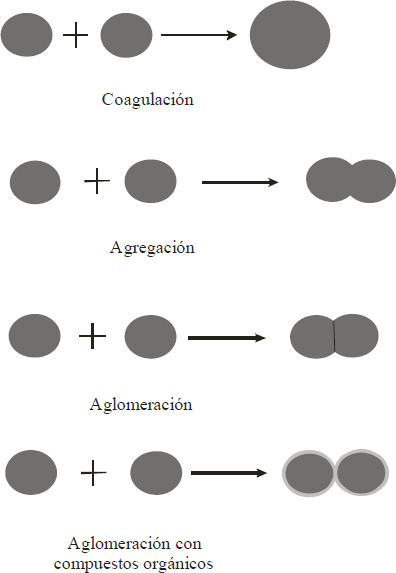
\includegraphics[width=0.6\textwidth]{UnionesParticulas.png}	 
	\caption{Representación de los tipos de uniones entre partículas primarias} \label{fig:unionesparticulas}
\end{figure} 

\par En la Figura \ref{fig:unionesparticulas} se esquematizan los tipos de uniones que pueden resultar de las colisiones a las que se pueden ver sometidas las partículas primarias en cualquier punto de la cámara de combustión o en el tubo de escape. A pesar de esta distinción, las palabras ?agregación? y ?aglomeración? suelen utilizarse indistintamente al describirse los distintos regímenes de crecimiento -no superficial- de las partículas, y las características morfológicas de éstas.

\par Posteriormente a las colisiones entre partículas primarias se pueden producir colisiones entre partículas primarias y aglomerados y/o colisiones entre aglomerados. Las colisiones entre partículas primarias y aglomerados se clasifican en los mismos tipos que las mostradas en la Figura \ref{fig:unionesparticulas}. Por otro lado las colisiones entre aglomerados provocan la formación de racimos cohesionados mediante fuerzas generalmente débiles, y donde la forma del aglomerado creado respeta la morfología de los aglomerados primogénitos.

\par El enracimamiento modifica el tamaño y estructura de las partículas, así como su capacidad de adsorción, su aerodinámica y su comportamiento óptico.	
\par En la cámara de combustión predominan las colisiones entre partículas primarias y entre pequeños agregados, aglomerados y partículas primarias, mientras que en el tubo de escape predomina el enracimamiento de aglomerados.
 
\subsection{Tipos de aglomeración}\label{sub:tiposaglomeracion}
\subsubsection{Introducción}

\par La simulación de los procesos de aglomeración requiere conocer el comportamiento espacial que tienen los aglomerados y cómo van formando aglomerados mayores y por tanto desapareciendo los de menor tamaño. Las hipótesis que hay que tener en cuenta se deben por un lado al propio movimiento de los aglomerados y por otro lado las debidas al propio proceso de colisión. El movimiento del aglomerado en el fluido requiere del estudio de toda la fluidodinámica de la partícula en el seno del fluido, cuestión que no se trata en esta tesis. Los tipos de colisiones que se pueden dar entre los aglomerados, aparte de la coagulación y la agregación, los resume P. Meakin et al \cite{meakinetal:1989}, y son:

\begin{itemize}
\item Aglomeración limitada por difusión.
\item Aglomeración balística.
\item Aglomeración limitada por reacción.
\end{itemize}

\par Los tres tipos de aglomeraciones anteriores a su vez se subdividen en dos, aglomeración partícula-racimo y aglomeración racimo-racimo, de manera que existen 6 formas distintas de formación de aglomerados.

\par Cuando las partículas son muestreadas en el tubo de escape (lejos ya de la zona de reacción), la estructura que presentan puede ser debida a aglomeración balística o a aglomeración limitada por difusión, dependiendo de la temperatura del gas de escape, del recorrido libre medio entre partículas y del tamaño de éstas, \cite{skillasetal:1998}, y por tanto de las condiciones de operación del motor.

\subsubsection{Aglomeración limitada por difusión} \label{subsub:Aglomeracionlimitadadifusion}

\par La aglomeración limitada por difusión es la denominada DLA (\textit{Diffusion-Limited Aggregation} o \textit{Agglomeration}). Si el camino libre medio entre los aglomerados o entre el aglomerado y la partícula primaria es pequeño frente al tamaño de las partículas, entonces la colisión entre las partículas es poco energética. En este caso las partículas se unen por uno o varios puntos de contacto sin perder su forma original. El contacto se produce por movimiento difusivo, básicamente. Si la aglomeración es del tipo partícula-racimo, entonces se demuestra que el aglomerado resultante tiende a una formación simétrica respecto a su centro de gravedad, de manera que las partículas se van aglomerando al racimo original de forma radial. El racimo crece simétricamente, tomando una forma de esfera porosa. Se demuestra que la dimensión fractal, que se define más adelante, tiende a 2.5, \cite{friedlander:2000}. 

\par El otro caso es el de colisión entre dos racimos cualesquiera que se denomina DLCA (\textit{Diffusion-Limited Cluster Aggregation} o \textit{Agglomeration}). En este caso los racimos recorren un camino aleatorio antes de colisionar, de manera que colisionan por uno o varios puntos. Después de la colisión los racimos originales permanecen inalterables en forma. Con este tipo de colisiones se consiguen aglomerados muy enracimados tendiendo a estructuras con forma de cadenas. La dimensión fractal media tiende a 1.8, \cite{megaridisetal:1990}.

\subsubsection{Aglomeración balística}

\par En el proceso de colisión balística, el camino libre medio entre las partículas que colisionan es muy grande respecto al tamaño de ambas partículas. Por ello, la energía cinética de las partículas es muy grande en el momento de la colisión. Este tipo de aglomeración es caracterizada porque las trayectorias trazadas por las partículas son muy rectilíneas, a diferencia de las colisiones DLA, en las que las trayectorias son de tipo aleatorio.

\par Si la aglomeración es entre una partícula primaria y un racimo, entonces la partícula primaria impacta contra el racimo introduciéndose dentro de él, ya que la energía cinética es elevada en el momento del impacto. El aglomerado tiende a ser una esfera más compacta, de manera que la dimensión fractal tiende a 3.0. 

\par Si la aglomeración se produce entre dos racimos, entonces se incrustan uno en otro produciendo un aglomerado de tipo cadena con una dimensión fractal superior que en el caso de una aglomeración de tipo DLA. En este caso la dimensión fractal tiende a 1.95, \cite{megaridisetal:1990}.

\subsubsection{Aglomeración limitada por reacción}

\par En los dos casos anteriores todas las colisiones producen un aglomerado de mayor dimensión, desapareciendo los dos aglomerados originales. En este caso, RLA (Reaction Limited Aggregation o Agglomeration), para que se forme un aglomerado nuevo, los dos aglomerados originales, además de contactar, deben superar alguna fuerza exterior, como puede ser la debida a cargas eléctricas ó potenciales químicos. De esta manera, para que dos aglomerados colisionen, la energía de colisión tiene que ser superior que en los dos casos anteriores. Si la aglomeración es entre una partícula primaria y un racimo, el aglomerado resultante tiende a ser una esfera compacta, cuya dimensión fractal tiende a 3.0. En el caso de aglomeración entre dos racimos, la dimensión fractal tiende a ser superior a 2.0, según P. Meakin et al \cite{meakinetal:1989} la dimensión fractal tiende a 2.09.

\subsection{Reestructuracion térmica del aglomerado}

\par La reestructuración térmica de las partículas depende del nivel térmico inicial y de la velocidad de enfriamiento. El nivel térmico inicial afecta directamente a la reestructuración térmica. Cuanto mayor sea el nivel térmico inicial mayor será la reestructuración térmica de las partículas. Por otro lado, la velocidad de enfriamiento afecta inversamente a la reestructuración térmica. Cuanto mayor es la velocidad de enfriamiento, menor es el tiempo de residencia a alta temperatura, y como consecuencia menor es la posibilidad de que exista reestructuración térmica.

\par Dependiendo de la estructura interna del aglomerado, la reestructuración térmica puede afectar a las partículas de dos maneras distintas:

\begin{itemize}
\item Si las partículas primarias que componen el agregado o aglomerado están fuertemente unidas unas a otras, pueden conservar durante su exposición a las altas temperaturas su tamaño medio, caso nº 1 de la Figura \ref{fig:reestructuraciontermica}. En este caso, el tamaño y la forma estructural del agregado tienden a conservarse, mientras que los tamaños medios de las partículas primarias aumentan debido al crecimiento superficial de las partículas primarias, \cite{sempereetal:1993}. Como consecuencia la dimensión fractal tiende a aumentar.

\item Si las partículas primarias que conforman el aglomerado están unidas mediante fuerzas débiles, la exposición a las altas temperaturas puede llevar consigo una reestructuración del aglomerado haciendo que se vuelva más compacto y por tanto aumente su dimensión fractal, \cite{stasio:2001}, \cite{dalisetal:2005}. En este caso, existe reestructuración morfológica sin necesidad de que las partículas primarias sufran crecimiento superficial, ya que éstas varían su posición interna en el aglomerado, \cite{schmidt:1988,liuetal:2004}. Esta reestructuración se muestra en el caso nº 2 de la Figura \ref{fig:reestructuraciontermica}.

\end{itemize}

\begin{figure}[ht]
\centering
	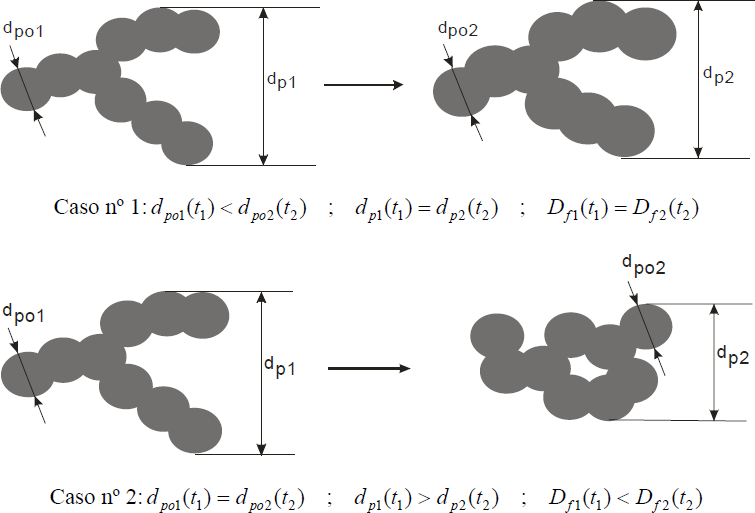
\includegraphics[width=0.6\textwidth]{ReestructuracionTermica.png}	 
	\caption[Tipos de reestructuración térmica de los aglomerados]{Tipos de reestructuración térmica de los aglomerados.Los subíndices 1 y 2 indican los estados previo y posterior a la reestructuración térmica} \label{fig:reestructuraciontermica}
\end{figure} 

\par El primer tipo de reestructuración térmica puede suceder dentro de la cámara de combustión donde la elevada temperatura favorece la fusión de pequeñas partículas sobre la superficie de los aglomerados. El segundo tipo de reestructuración térmica se puede dar, tanto en la cámara de combustión como en el tubo de escape, si bien es el tipo de reestructuración que predomina en el tubo de escape.
\par En ambos casos, la reestructuración térmica lleva consigo un cambio en la anisotropía y en el área proyectada de los aglomerados, ya que varía la conformación geométrica de los mismos, \cite{mikhailovetal:1996}.
\par Por otra parte, dependiendo de la forma del aglomerado y del tamaño de las partículas primarias que lo componen, la velocidad de enfriamiento de la partícula varía, ya que ésta depende principalmente de su área superficial, \cite{liuetal:2004}.
 
\section{Diámetros Equivalentes y Funciones de Distribución}\label{sec:diametrosyfuncionesequivalentes}

\subsection{Diámetros Equivalentes} \label{sub:diametros}

\par Se puede definir el diámetro equivalente de una partícula como el diámetro de la esfera que tendría el mismo valor de una propiedad física particular que la partícula irregular considerada. De esta manera, en función de la propiedad física fijada se define el diámetro equivalente considerado, \cite{friedlander:2000}.

\par En el esquema de la Figura \ref{fig:propiedadesparticulas} se presentan algunas propiedades físicas de las partículas relacionadas con el diámetro junto con el rango de tamaños en el que tal medida es posible o en el que se mantiene tal relación.

\par Se muestra en la Figura \ref{fig:propiedadesparticulas} que la resistencia del medio al movimiento de las partículas, la velocidad de evaporación y la velocidad de enfriamiento son proporcionales al cuadrado del tamaño de las partículas, si éstas son del orden de pocos nanómetros, \cite{fuchs:1989}. En cambio, estas propiedades físicas son proporcionales al tamaño de las partículas cuando éstas tienen un tamaño del orden de micrómetros. La frecuencia de colisiones con coagulación tiene su máximo cuando las partículas tienen un tamaño del orden de pocos nanómetros. La dispersión de luz por las partículas es proporcional al tamaño de éstas elevado a la sexta potencia, si el tamaño de las partículas es de pocos nanómetros. En cambio, si el tamaño de las partículas es del orden de micrómetros, la dispersión de luz es proporcional al cuadrado del tamaño de las mismas, \cite{fuchs:1989}.

\par También se muestra en la Figura \ref{fig:propiedadesparticulas} la región de visibilidad microscópica, por medio de microscopios ópticos, que está en el orden de micrómetros, y la región de visibilidad ultramicroscópicas, por medio de microscópicos electrónicos, que puede incluso llegar a pocos nanómetros. Por último, se muestra en la Figura \ref{fig:propiedadesparticulas} que el movimiento de partículas con tamaños de pocos nanómetros es predominantemente difusivo, mientras que el movimiento de partículas con tamaños del orden de micrómetros es predominantemente convectivo o de sedimentación.

\begin{figure}[ht]
\centering
	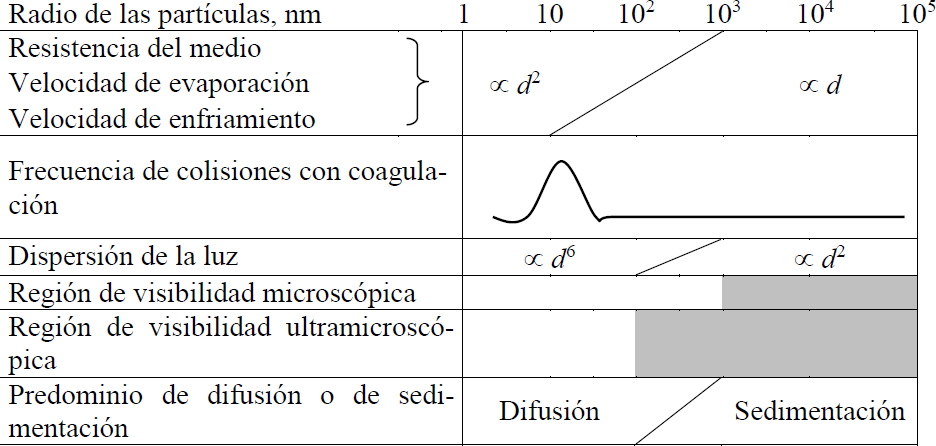
\includegraphics[width=0.9\textwidth]{PropiedadesParticulas.png}	 
	\caption{Algunas propiedades de las partículas en relación a su tamaño} \label{fig:propiedadesparticulas}
\end{figure} 

\par Normalmente las propiedades físicas de las partículas irregulares son muy difíciles de medir, y dependiendo de la propiedad física y con la tecnología actual, incluso pueden ser imposibles de medir. Por lo tanto, los diámetros equivalentes que se suelen definir son los que se pueden medir experimentalmente.

\par El diámetro aerodinámico es uno de los más comunes. Se define como aquel diámetro que tiene una partícula esférica de densidad unitaria, 1 $gcm^{-3}$, cuya velocidad de sedimentación o deposición es igual a la partícula irregular en cuestión. El diámetro aerodinámico se mide en ciclones e impactadores, \cite{smekensetal:1997}. Esta definición de diámetro no tiene en cuenta las trayectorias de las partículas, de manera que para partículas muy pequeñas las trayectorias pueden ser muy irregulares o incluso caóticas. Para este tipo de partículas el movimiento se caracteriza por ser predominantemente difusivo, Figura \ref{fig:propiedadesparticulas}. 

\par Se define diámetro equivalente de Stokes como el de una partícula esférica que tiene la misma resistencia aerodinámica que la partícula irregular si la partícula tiene una velocidad diferente a la del fluido portador, \cite{hinds:1982}. El diámetro equivalente de Stokes no depende de la densidad de la partícula, ya que la resistencia aerodinámica depende de la densidad del fluido, del coeficiente aerodinámico, del área frontal de la partícula y de la velocidad relativa entre la partícula y el fluido.

\par Se define el diámetro equivalente de movilidad eléctrica como el diámetro de una esfera con igual diámetro de Stokes que la partícula irregular y que además tenga la misma carga eléctrica. De esta manera, partículas con diámetros de Stokes iguales y que además lleven idéntica carga eléctrica, tienen igual movilidad eléctrica. El diámetro de movilidad eléctrica se puede medir experimentalmente con un SMPS (Scanning Mobility Particle Sizer), \cite{vangulijketal:2004}.

\par Las partículas de igual diámetro de Stokes que llevan idéntica carga eléctrica, tienen la misma movilidad eléctrica. Si además el campo eléctrico es unitario, el diámetro de Stokes y el diámetro equivalente de movilidad eléctrica se igualan.

\par El diámetro de giro es el diámetro de un anillo toroidal que tiene la misma inercia que la que tiene la partícula irregular. La ventaja de utilizar esta definición de diámetro característico radica en que es un parámetro puramente geométrico que sólo depende de la posición espacial de las partículas primarias que componen el aglomerado. Otros autores como K.H. Naumann \cite{naumann:2003} lo denominan diámetro geométrico de la partícula irregular.

\par El diámetro másico equivalente es el diámetro de una esfera que tiene la misma masa que la partícula irregular, \cite{naumann:2003}. Este diámetro es muy difícil de medir directamente, por lo que se determina a partir de otras variables como el diámetro de giro.

\par El diámetro del volumen equivalente es el diámetro de una esfera que tiene el mismo volumen que la partícula irregular, \cite{parketal:2003}.

\par El diámetro de proyección equivalente es el diámetro de una esfera que tiene el mismo área proyectada que la partícula irregular, \cite{whitby:1978}. 

\subsection{Funciones de Distribución}\label{subsec:funcionesdistribucion}

\par El hollín en el gas de escape de un motor diésel es un aerosol polidisperso, es decir, cubre un amplio rango de tamaños de partículas. La función que caracteriza el número de partículas que tienen un determinado tamaño se denomina función de distribución de tamaños. 
La clasificación modal propuesta por K.T. Whitby \cite{whitby:1978} es la más utilizada para clasificar las partículas del aerosol atmosférico. La clasificación modal se resume en la Figura \ref{fig:distribuciontipicaparticulas} La línea continua indica la concentración de partículas en el gas de escape en número, y la línea discontinua indica la concentración másica de las partículas diésel.

\par Como se muestra en la Figura 2.6 las funciones de distribución siguen funciones del tipo logarítmico-normales presentando normalmente tres modas. Las tres modas son la moda núcleos, acumulación y gruesa, \cite{kittlesonetal:1998}. La moda núcleos está comprendida entre pocos nanómetros, 5 nm, a 50 nm, aproximadamente. La moda acumulación está comprendida entre 50 nm y 1000 nm, mientras que la moda gruesa son partículas mayores a 1000 nm.

\par La función de distribución logarítmico-normal corresponde con la siguiente expresión, tomada de \cite{friedlander:2000}:

\begin{equation}
\label{ec:distribucionlogaritmico-normal}
f(d_p)\,=\,\dfrac{1}{\sqrt{2 \pi} d_p ln(\sigma)} exp\left( -\dfrac{1}{2 ln^2 \sigma} \left( lnd_p - ln \overline{\overline{d_p}} \right)^2 \right)
\end{equation}

donde $\sigma$ es la desviación estándar geométrica y $\overline{\overline{d_p}}$ es el diámetro medio geométrico de la función de distribución. La desviación típica geométrica y el diámetro medio geométrico se calculan mediante las siguientes ecuaciones:

\begin{align}
\label{ec:desviaciontipicageometrica}
ln(\overline{\overline{d_p}}\, & =\,\overline{lnd_p}\,=\,\int_0^\infty lnd_p f(d_p) dd_p \\
\label{ec:diametromediogeometrico}
ln^2 \sigma\, & =\,\overline{\left(ln d_p - ln \overline{\overline{d_p}} \right)^2}\,=\, \int_0^\infty \left( lnd_p - ln \overline{\overline{d_p}} \right)^2 f(d_p)dd_p
\end{align}

\par Este diámetro se puede asociar a cualquiera de las definiciones que se han presentado en el epígrafe \ref{sub:diametros}.

\par Otra función de distribución utilizada es la logarítmico-normal bimodal, que recoge las modas nuclear y acumulativa por medio de una sola función \cite{kazakovetal:1998},

\begin{equation}
\label{ec:logartimico-normalbimodal}
f(d_p)\,=\,\dfrac{1}{3\sqrt{2} \pi d_p}\left[ \dfrac{a}{ln \sigma_1} exp\left( - \dfrac{\left( lnd_p - ln \overline{\overline{d_{pl}}} \right)^2}{18ln^2 \sigma_1} \right)  + \dfrac{1-a}{ln \sigma_2}exp\left( - \dfrac{\left( lnd_p - ln \overline{\overline{d_{p2}}} \right)^2}{18ln^2 \sigma_2} \right) \right]
\end{equation}

donde los subíndices 1 y 2 representan las dos modas y $a$ es un parámetro de ajuste que expresa la separación entre las dos modas.

\section{Efectos mediambientales y fisiológicos}
\subsection{Introducción}
\par La emisión de partículas constituye uno de los mayores problemas medioambientales atribuidos a los motores diésel. El trabajo europeo APHEIS \cite{apheis:2004}, recientemente, ha cuantificado los efectos de la emisión de partículas diésel sobre la salud, en términos de mortalidad prematura y de ingresos en los hospitales. Adicionalmente, la absorción de radiación por las partículas de hollín en todo el rango de longitudes de onda de la radiación solar es conocido y además influye apreciablemente en el clima, \cite{sorensen:2001}.

\par Se sabe que la irregularidad de la partícula diésel afecta directamente al impacto medioambiental y a la salud pública por varias razones:
 
\begin{itemize}
\item Cuanto más irregulares son las partículas mayor es la relación entre el área superficial y el volumen, haciendo que aumente la capacidad de absorción de hidrocarburos. 

\item La irregularidad de las partículas afecta directamente a la capacidad que tienen éstas de extinguir la radiación luminosa incidente sobre ellas, por lo que afecta a la opacidad del gas portador de las partículas, haciendo que ésta aumente.

\item La irregularidad de las partículas afecta al comportamiento aerodinámico de éstas, ralentizando su velocidad de sedimentación y aumentando, por tanto, su probabilidad de entrar en las vías respiratorias humanas.

\item La irregularidad de las partículas aumenta la eficiencia de filtrado de los sistemas de retención de partículas tanto artificiales como las propias del cuerpo humano, \cite{bockhornetal:2002}. Concretamente tiene especial interés el conocimiento de la morfología de las partículas para el diseño de los sistemas de postratamiento de los gases de escape del motor diésel (Trampas de partículas).

\end{itemize}

Otros efectos asociados a la irregularidad de las partículas diésel son los referentes a las propiedades del transporte, como son la difusión energética y de cantidad de movimiento, y las propiedades de radiación de calor, etc. \cite{meakinetal:1989}. 
La manera más común de cuantificar la irregularidad de las partículas es mediante la dimensión fractal, como se explica en B.B. Mandelbrot \cite{mandelbrot:1983}. Algunos autores como R.J. Samson et al \cite{samsometal:1987}, C. Van Gulijk et al \cite{vangulijketal:2004}, A.V. Filippov et al \cite{filippovetal:2000}, K.O. Lee et al \cite{leeetal:2003}, han utilizado esta manera de cuantificar la irregularidad para muchos ejemplos de gran interés práctico.

\subsection{Parámetros para caracterizar emisiones} \label{sub:parametroscaracterizaremisiones}

\subsubsection{Índice de emisión}

\par El índice de emisión para la especie contaminante $i$ es la relación entre la masa de dicha especie y la masa de combustible quemado por el proceso de combustión.

\begin{equation}
\label{ec:indiceemision}
EI_i\,=\, \dfrac{m_i}{m_f}
\end{equation}

\par Como se puede observar, el índice de emisión es adimensional. Sin embargo, para valores muy pequeños de dicho índice, suelen utilizarse unidades como, por ejemplo, $g/kg$. Este índice es muy útil en el sentido en que no da lugar a ambigüedad en su interpretación ya que expresa la cantidad de contaminante formado por masa de combustible consumido, independientemente del grado de dilución de los productos o de la eficiencia de la combustión.

\par En la combustión de un hidrocarburo con aire, el índice de emisión puede ser calculado a partir de la medida de las concentraciones de las especies de interés junto con todas aquellas especies que contienen carbono. Asumiendo que todo el carbono del combustible aparece como $CO$ y $CO_2$ en los productos de la combustión, se puede escribir la ecuación \ref{ec:indicecombustiontotal}

\begin{equation}
\label{ec:indicecombustiontotal}
EI_i\,=\,\left( \dfrac{X_i}{X_{CO}+XO_{CO_2}} \right) \left( \dfrac{nPM_i}{PM_f} \right)
\end{equation}

donde X son las fracciones molares, n es el número de átomos de carbono en un mol de combustible CnHm y PMi y PMf son los pesos moleculares de la especie i y del combustible respectivamente. El primer término de la ecuación (15.2) representa el número de moles de i por mol de carbono del combustible, mientras que el segundo término permite la conversión de moles de carbono a moles de combustible y su respectiva conversión a unidades másicas. 

\par En un proceso de combustión de una mezcla pobre (condiciones de trabajo con exceso de aire), en el cual las cantidades de $CO$, $H_2$, y otras especies contaminantes, sean muy pequeñas, la combustión de un mol de combustible con aire (suponiendo que el aire es una mezcla con un 21\% de $O_2$ y un 79\% en volumen de $N_2$) se puede expresar como se muestra en :

\begin{equation}
\label{ec:combustionpobre}
C_nH_mO_p + aO_2 +3.76aN_2 \rightarrow nCO_2+ \left( \dfrac{m}{2} \right)H_2O+aO_2+3.76aN_2
\end{equation}

\par La fracción molar para la especie $i$ se define como: 

\begin{equation}
\label{ec:fraccionmolar}
X_i\,=\, \dfrac{n_i}{n_t}\,=\, \dfrac{n_i}{n_{CO_2}+n_{H_2O}+n_{N_{2(a)}}}\,=\, \dfrac{n_i}{n+\frac{n}{2}+3.76aN_2}
\end{equation}

\par Es importante señalar que la relación anterior se refiere a un proceso de combustión con mezcla pobre (exceso de aire). Para mezclas ricas, la situación es más complicada debido a que las cantidades de monóxido de carbono y de hidrógeno molecular son mucho más importantes y, por lo tanto, se han de contabilizar en los moles totales de productos de la combustión. De forma general, se puede escribir que:

\begin{equation}
\label{ec:fraccionmolargeneral}
X_i\,=\, \dfrac{n_i}{n_t}
\end{equation}

\subsubsection{Medidas típicas de emisiones}
\par Los niveles de emisión pueden expresarse de distintas formas que a veces pueden dar lugar a comparaciones dificultosas y ambiguas. Estas diferencias tienen su origen en las necesidades de las distintas tecnologías \cite{turns:1996}. En vehículos pesados diésel y de gasolina, resulta común expresar las emisiones en función de la potencia efectiva suministrada por los mismos (emisión específica) como:

\begin{equation}
\label{ec:emisionespecifica}
EE_i\,=\, \dfrac{\dot{m_i}}{N_e}
\end{equation}

En esta expresión \ref{ec:emisionespecifica} las unidades normalmente utilizadas son $g/kWh$. La emisión específica está relacionada con el índice de emisión (EI) por la siguiente ecuación: 

\begin{equation}
\label{ec:EI}
EE_i\,=\, \dfrac{\dot{m_i}}{N_e}\,=\, \dfrac{\dot{m_f}EI_i}{N_e}
\end{equation}

\par Otra medida de las emisiones frecuentemente empleada es la masa de contaminante emitida por unidad de energía liberada por el combustible \ref{ec:masaemitida}, donde PCI es el poder calorífico del combustible:

\begin{equation}
\label{ec:masaemitida}
\dfrac{\dot{m_i}}{Q_{lib}}\,=\, \dfrac{EI_i}{PCI}
\end{equation}

\par Las unidades usuales son $g/MJ$. 

\par En vehículos ligeros, suele usarse la cantidad de contaminante emitida por la distancia recorrida por el vehículo (g/km). Sin embargo, para procesos de homologación, la medida viene dada en g/ciclo de homologación. 

\par En muchas ocasiones resulta ventajoso expresar las emisiones en unidades adimensionales. Las unidades más comúnmente utilizadas son el tanto por uno o tanto por ciento, las partes por millón (bien en masa o bien en volumen, siendo el factor de conversión de una a la otra el peso molecular) y si las cantidades emitidas son muy pequeñas, en partes por billón (que también pueden referirse a la masa o al volumen). Si las emisiones son gaseosas, lo más habitual es que dichas unidades se refieran a relaciones volumétricas, coincidiendo entonces con las relaciones molares.

\par En resumen, se pude afirmar que la medida utilizada depende cual sea la aplicación específica del proceso. 

\subsection{Efectos sobre la salud pública}

\par Durante la respiración humana no sólo se inhala oxígeno, nitrógeno y el resto de gases que componen el aire, sino que además entran en las vías respiratorias todas las partículas que están en suspensión en el aire. Las partículas con diámetros menores a $2.5 \mu m$ se llaman partículas finas y tienen una deposición alveolar pequeña ya que son interceptadas o filtradas con anterioridad en la parte bronquial. El problema está con las partículas ultrafinas, de tamaño inferior a 100 nm, que sí llegan a la región alveolar y además la tasa de deposición alveolar es muy elevada, \cite{leeetal:2003}, como puede verse en la Figura \ref{fig:deposicionalveolar}.

\begin{figure}[ht]
\centering
	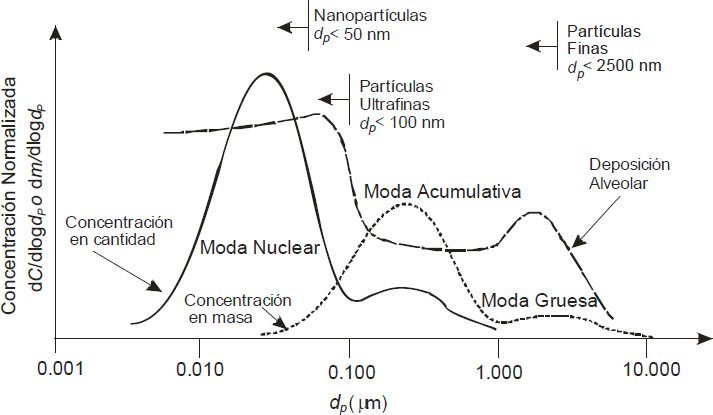
\includegraphics[width=0.9\textwidth]{DeposicionAlveolar.png}	 
	\caption{Deposición alveolar de las partículas diésel en función de su tamaño, adaptado de D.B. Kittelson \cite{kittleson:1998} y de J.M. Desantes et al \cite{desantesetal:2005}.} \label{fig:deposicionalveolar}
\end{figure} 

\par El problema de la deposición alveolar de las partículas ultrafinas, se agrava por la mayor concentración de éstas en el aire. Los motores diésel actuales producen mayor número de partículas ultrafinas que sus predecesores, si bien no existen correlaciones evidentes entre el tipo de motor diésel y su antigüedad con el tipo de partículas emitidas, \cite{morawskaetal:1998}.

\par El humo producido por los motores diésel tiene menor tasa de deposición en los pulmones que el producido por el tabaco y que el producido por los motores de gasolina, \cite{morawskaetal:1998}. Este estudio experimental comprobó que la tasa de deposición del humo de un motor diésel sobre los pulmones es del 30\%, frente a la del humo del tabaco que es del 36\% y la del humo de un motor de gasolina, que es del 41\%. Estas cifras no son directamente proporcionales a los tamaños medios de movilidad de las partículas que son para el humo del tabaco de 183 nm, para el humo de un motor diésel de 125 nm y para el humo de un motor de gasolina de 69 nm. Tampoco son iguales las tendencias de la tasa de deposición pulmonar al variar el tamaño de las partículas: por ejemplo, la tasa de deposición del humo de tabaco apenas se ve afectada por el tamaño de las partículas, mientras las de los humos de los motores disminuyen al aumentar los tamaños. Los autores atribuyen tales diferencias precisamente a la diferente morfología de las partículas y de las unidades esféricas que las componen (mucho mayores en el caso del humo del tabaco), y señalan mecanismos como la deposición en bifurcaciones bronquiales, que afectan mucho más a las estructuras enracimadas que a las compactas, como puede comprobarse en la Figura \ref{fig:comparativafotos}.
  
\begin{figure}[ht]
\centering
	 \subfloat[Fotografía de un aglomerado diésel típico]{\label{subfig:particuladiesel}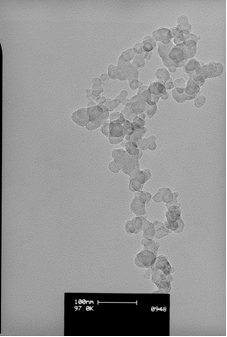
\includegraphics[scale=0.9]{Fotoparticuladieseltipica.png}}
	 \qquad
	 \subfloat[Fotografía de una partícula de humo de tabaco]{\label{subfig:particulahumotabaco}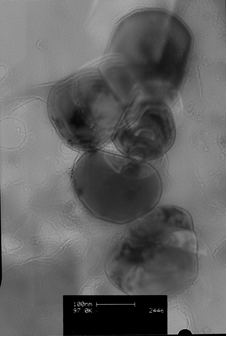
\includegraphics[scale=0.9]{Fotohumotabaco.png}}
	 \caption{Fotografía de una partícula diésel típica \ref{subfig:particuladiesel}. Fotografía de una partícula perteneciente al humo del tabaco\ref{subfig:particulahumotabaco}}
\end{figure} \label{fig:comparativafotos}

\par Otros efectos que pueden producir las partículas sobre la salud humana son los derivados de la propia naturaleza de estas partículas y de los distintos compuestos químicos que pueden llevar absorbidos en su superficie. G. Oberdörster \cite{oberdoster:2001} y A. Seaton et al \cite{seatonetal:1995} constataron que la inhalación de partículas lleva consigo la inflamación de las vías respiratorias, provocando un considerable daño en las mismas y en el sistema cardiovascular. La parte soluble de la partícula puede traspasar la membrana alveolar pasando a la sangre y distribuyendo su toxicidad por todo el cuerpo, mientras que la parte insoluble se queda alojada en las vías respiratorias, disminuyendo, por tanto la capacidad respiratoria. Por otro lado las partículas están compuestas por PAH (Polycyclic Aromatic Hydrocarbons) que son compuestos cancerígenos, \cite{benneretal:1990}. Todos estos efectos son, por tanto, consecuencia indirecta de la morfología de las partículas, en la medida en que ésta influye decisivamente sobre la probabilidad de inhalación de las mismas, y sobre la capacidad de absorción de sustancias tóxicas.

\subsection{Impacto medioambiental}

\par El impacto medioambiental de las partículas diésel es muy diverso. Las partículas juegan un papel muy importante en la contaminación ambiental y pueden tener un posible efecto sobre el cambio climático, \cite{przybiolla:2002}, \cite{petterssonetal:2004} y \cite{chameidesetal:2002}.

\par Las nubes son pequeñas gotas de agua formadas a partir de la condensación del vapor de agua alrededor de un núcleo ya condensado. Las partículas en suspensión son base o núcleos alrededor de los cuáles puede condensar vapor de agua, promoviendo la formación de nubes con consecuencias climáticas adversas, \cite{zhangetal:2006}. El hollín en suspensión incrementa la dispersión y la absorción de la radiación solar, \cite{ackermanetal:2000}, y reduce la radiación solar que incide sobre la superficie terrestre, afectando por consiguiente el clima terrestre, \cite{menonetal:2002}. Además, puede alterarse la estructura térmica de la atmósfera, reduciendo la probabilidad de lluvias y haciendo, por tanto, menos eficiente la eliminación de contaminantes de la atmósfera, \cite{ramanathanetal:2001}.

\par Existe un fenómeno llamado gravito-fotofóresis por el cuál las partículas tienden a subir en la atmósfera hasta alcanzar alturas desde 20 km hasta 83 km, \cite{cheremisinetal:2005}. De esta forma, las partículas quedan suspendidas en la atmósfera según su tamaño. Las más pequeñas quedan en capas superiores y las de tamaño entorno al micrómetro, en capas más bajas de la atmósfera. La presencia de estas capas aumenta tanto la reflexión de la luz solar incidente sobre el planeta, como la dispersión de luz. Al margen de la consecuente disminución de visibilidad, este efecto puede ser tan grande que puede disminuir el flujo neto de energía solar que llega a la corteza terrestre, \cite{faxvogetal:1978}, provocando un enfriamiento en ésta, opuesto al efecto invernadero. Este efecto es más intenso cuanto mayor es la emisividad de la superficie terrestre. Por el contrario, cuando la superficie terrestre es brillante, las capas de partículas dificultan la reflexión provocando un efecto similar y potenciando el efecto invernadero. Coincide, además, que la potenciación del efecto invernadero tiene lugar en zonas más cálidas y desérticas (con superficies más reflectantes) y el enfriamiento superficial, en las zonas más frías y húmedas (por lo general más absorbente). En cualquiera de los dos casos el carácter regional o zonal de este efecto, frente al global del efecto invernadero hace que, más que mitigar o potenciar éste, el efecto más notable de la presencia de las capas de partículas sea el de dificultar la observación del efecto invernadero. El comportamiento óptico de las partículas, responsable de los fenómenos descritos, depende mucho del tamaño y de la irregularidad de las partículas y de la posible presencia en su superficie de hidrocarburos condensados, \cite{siegmannetal:1999}.

\par Por otra parte, las partículas son portadoras de sustancias que pueden reaccionar con los distintos gases de la atmósfera o que pueden catalizar reacciones no deseadas en el ambiente, \cite{merolaetal:2001}. Por ejemplo las partículas de hollín pueden contener $SO_2$, el cual puede reaccionar con el agua y producir ácido sulfúrico. El ácido sulfúrico es arrastrado por la lluvia haciendo que ésta sea muy corrosiva, lo que se denomina lluvia ácida.

\par El impacto medioambiental de las partículas diésel depende directamente de la concentración, de la irregularidad, del tamaño y de la eficiencia a la extinción de luz de las partículas que estén en suspensión en el ambiente. El tiempo medio de residencia en suspensión es mayor cuanto mayor es la irregularidad de las partículas y cuanto menor es el tamaño de éstas, por lo que cuanto mayor es la irregularidad de las partículas y menor el tamaño de éstas, mayor es el impacto medioambiental de las partículas diésel. Igualmente, cuanto mayor es la eficiencia a la extinción de luz de las partículas menor es la visibilidad y mayor es el impacto medioambiental, en cualquiera de las dos formas mencionadas. 
 
\newpage
\bibliographystyle{Config/ealpha}		
\bibliography{Chapters/Bibliografia}
		\chapter{MÉTODOS DE ANÁLISIS FRACTAL}\label{cap:MetodosAnalisisFractal}
%\vspace{0.1cm}
\noindent\rule{\linewidth}{1.3pt}\\
\startcontents[chapters]
\printcontents[chapters]{}{1}{}
%\vspace{0.1cm}
\noindent\rule{\linewidth}{1.1pt}\\
%\minitoc
\newpage
\section{Geometría fractal}\label{sec:GeometriaFractal}
\section{Conceptos básicos}\label{sec:ConceptosBasicosDimension}
<<<<<<< HEAD
\par Las partículas emitidas en procesos de combustión, bien sean en llamas en hornos, quemadores o en motores diésel, forman conjuntos de partículas llamados \index{aglomerados} \emph{aglomerados}. Cada partícula constituyente de dicho aglomerado se denomina \index{partícula primaria} \emph{partícula primaria}. Asimismo, los aglomerados formados en las tecnologías que involucran suspensiones sólidas coloidales están formados a menudo por partículas primarias \index{monómeros}(\emph{monómeros}) con formas parecidas a \index{esférulas} \emph{esférulas}, cuyos diámetros son muy uniformes en tamaño. Algunos procesos de formación de partículas tienen como resultado final la obtención de productos diferentes a los de partida. Tal es el caso de la industria de los pigmentos. Mientras, otros procesos generan subproductos, siendo la formación de hollín en el conducto de escape de un motor Diésel un ejemplo de estos últimos. Aunque los procesos de formación puedan ser muy diferentes, la formación de partículas de SiO$_2$ y TiO$_2$ llevan a la formación de partículas cuya apariencia física es muy parecida. Estos son sólo dos ejemplos de una amplia variedad de entornos industriales cuyos procesos conllevan la formación de aglomerados con morfologías que no sólo son similares, sino que también sus propiedades son muy similares las unas de las otras, con independencia del material de entrada al proceso. Las propiedades resultantes dependen fuertemente de la disposición espacial y la morfología, la cual tiene un fuerte impacto en las propiedades finales de los aglomerados.

\par El último es el caso de los aglomerados de hollín diésel, entre otros \cite{lapuertaetal:2007}. En los estudios de simulación, es común asumir un diámetro uniforme para las partículas primarias, \cite{wuetal:1993,tandonetal:1995,ohetal:1997,leeetal:2002,zhuetal:2003}, ya que se ha probado que la polidispersidad no afecta significativamente a los parámetros morfológicos que describen el aglomerado \cite{busheletal:1998}. Estas partículas primarias se disponen en el aglomerado formando racimos irregulares con tamaños, formas y masas diferentes los unos de los otros. Pueden considerarse como estructuras cuasifractales y se acepta que, en el caso de estar compuestos por un número suficiente de partículas primarias pueden describirse mediante la \emph{Ley de Potencias}, siendo la \textbf{dimensión fractal} y el \textbf{prefactor} como los parámetros característicos \cite{bonczyketal:1991}. Los tamaños tan dispersos de los aglomerados, junto con los bien conocidos efectos medioambientales y sobre la salud que tiene la morfología de los aglomerados (no sólo con respecto al tamaño sino también con respecto a la forma) \cite{kittleson:1998,meakinetal:1989} hacen necesaria una descripción cuantitativa adecuada de los aglomerados de hollín.

\par La forma más común de cuantificar esta irregularidad es usando la dimensión fractal, adoptada de \cite{mandelbrot:1983} partiendo de la propuesta previa de Félix Hausdorff. La aplicación de una dimensión fractal a los aglomerados de hollín diésel supone asumir que estos aglomerados se corresponden con geometrías fractales. Aunque los aglomerados de hollín se pueden clasificar como racimos granulosos o granulares siguiendo la concepción original de Mandelbrot, se consideran usualmente estructuras cuasifractales, ya que no pueden ser ciertamente ser autosimilares (o autoescalares como las denominó Mandelbrot) a menos que estén compuestas de un número muy grande de partículas primarias.

\par En la literatura se han propuesto diferentes métodos experimentales para determinar la dimensión fractal de aglomerados de hollín a partir de sus imágenes planas obtenidas mediante \textit{Microscopio de Transmisión Electrónica} (TEM por sus siglas en inglés). El más común se basa en ajuste lineal del diámetro de giro frente al número de partículas primarias, en un diagrama log-log \cite{leeetal:2002}

\begin{equation}
\ln(n_{p_o})\,=\,\ln(k_{f})+D_{f}\ln(\frac{d_{g}}{d_{p_o}})
\label{eq:leydepotencias}
\end{equation}

\par Este método se deriva de la aplicación de la \index{Ley de Potencias}, la cual está considerada ampliamente como la ecuación característica que gobierna las estructuras fractales o cuasifractales \cite{samsometal:1987,caietal:1995,koyluetal:1995}, etc. La dimensión fractal \nomenclature{$D_{f}$}{Dimension Fractal} se obtiene entonces como la pendiente de la recta de regresión, mientras que el prefactor \nomenclature{$k_{f}$}{Prefactor de la Ley de Potencias} se identifica con el valor cuya abscisa es cero. Sin embargo, este método tiene cinco desventajas importantes:

\begin{enumerate}
	\item Es incapaz de dar una dimensión fractal y un prefactor para los aglomerados de forma individual. En cambio, da un valor medio de ambos parámetros para una población grande de aglomerados. Una descripción individual de la morfología del aglomerado abría las posibilidades de una mejor discriminación de los efectos de las condiciones operativas del motor, tipo de combustible utilizado, condiciones térmicas en el conducto de escape, etc. sobre el tamaño, forma y efectos potenciales medioambientales de las emisiones de hollín. Pocos métodos geométricos se han propuesto para la determinación individual de la dimensión fractal de aglomerados de hollín hasta la fecha \cite{lattuadaetal:2003,lapuertaetal:2006,wozniaketal:2012}.
	\item El número de partículas primarias que componen el aglomerado es desconocido, y se estima normalmente a través de otra Ley de Potencias distinta que intenta reproducir el solape entre partículas primarias cuando el aglomerado se proyecta en un plano, \cite{medaliaetal:1969,megaridisetal:1990}, \cite{brasiletal:1999,leeetal:2003}. Sin embargo, el exponente para esta Ley de Potencias adicional, $z$, no se determina de forma unívoca, ya que de hecho depende de la forma y tamaño del aglomerado \cite{ohetal:1997}. El solape y el aplastamiento no deben confundirse: el primero es un efecto visual de las partículas ocultas tras otras partículas en la proyección plana, mientras que el último es un efecto morfológico debido a la colisión de partículas primarias que resulta en geometrías que están lejos de ser esféricas.
	
	\begin{equation}
	\ln(n_{p_o})\,=\,\ln(z)+\ln(\frac{A_{p}}{A_{p_o}})
	\label{eq:leydepotenciassolape}
	\end{equation}
	
	\item El diámetro de giro del aglomerado se identifica normalmente con el diámetro de giro de su proyección plana \cite{rogaketal:1992,koyluetal:1995,ohetal:1997}, a pesar de que se ha probado que subestima el diámetro de giro del aglomerado tridimensional. Este error lleva a que los métodos basados en proyecciones de imágenes planas subestimen la dimensión fractal de las estructuras tridimensionales \cite{rogaketal:1992,nelsonetal:1990,adachieetal:2007}.
	
	\item Se supone tamaño uniforme para las partículas primarias. Esta suposición podría parecer muy restrictiva. De hecho, se puede probar que se puede obtener una distribución de tamaños estadística en todos los procesos que involucran interacción de partículas \cite{busheletal:1998}. Sin embargo, el asumir tamaño uniforme para modelar la morfología de los aglomerados constituidos por partículas primarias ha demostrado ser un enfoque correcto al problema.
	
	\item Las partículas primarias se asumen esféricas, sin tener en cuenta los efectos de aplastamiento, que podrían afectar al prefactor y a la dimensión fractal obtenidos \cite{ohetal:1997,brasiletal:1999,alzaitoneetal:2009}.
\end{enumerate}

\par La investigación doctoral que se desarrollará comienza desde la base del modelo propuesto por \cite{lapuertaetal:2006} e intenta resolver los inconvenientes 2 a 4 anteriormente mencionados. La primera parte de esta investigación se dedica al análisis fractal  basada no solamente en la forma de los aglomerados a partir de sus proyecciones planas, sino también a partir de su opacidad. La \emph{Ley de Beer-Lambert}, que proporciona la transmitancia lumínica de imágenes de sólidos en escala de grises, se uso como base para determinar el número de partículas primarias ocultas detrás de las visibles. A partir del número de partículas primarias de cada aglomerado individual, su masa, momento de inercia, diámetro de giro se determinaron su densidad aparente y su dimensión fractal sin hipótesis adicionales acerca del solape y sin extrapolación de patrones promedio. Esta metodología ha sido publicada en la revista \textit{Measurement Science and Technology} y se encuentra en el Apéndice \ref{app:BeerLambert} al final de esta tesis.

=======
>>>>>>> 693e9268ae27c63b8df483515d98b793d51de772
\subsection{Concepto de Dimensión}
\subsection{Dimensión fractal}
\section{Ejemplos de fractales}\label{sec:EjemplosFractales}
\section{Hipótesis del modelado fractal}\label{sec:HipotesisModeladoFractal}
\section{Métodos del análisis fractal}\label{sec:MetodosAnalisisFractal}
\subsection{Métodos de Box--Counting}
\subsection{Métodos Multifractales}
\subsection{Métodos de Sistemas Funciones Iteradas (IFS)}
\section{Aplicaciones prácticas del análisis fractal}
\subsection{Análisis fractal de partículas diésel}
\subsection{Ejemplos en las ramas de la Biología y de la Botánica}
\subsection{Ejemplos en las ramas de la Geología y de la Geofísica}


\newpage
\bibliographystyle{ealpha}	
\bibliography{Chapters/Bibliografia}
		\pagestyle{plain}
\chapter{INSTALACIONES EXPERIMENTALES}\label{cap:InstalacionesExperimentales}
\vspace{0.2cm}
\noindent\rule{\linewidth}{1.5pt}\\
\startcontents[chapters]
\printcontents[chapters]{}{1}{}
\vspace{0.2cm}
\noindent\rule{\linewidth}{1.3pt}\\
%\dominitoc
\newpage
\section{Instalaciones de la UCLM}\label{sec:InstalacionesUCLM}
\section{Instalaciones de la UMA}\label{sec:InstalacionesUMA}
\section{Resumen}
\newpage
\bibliographystyle{Config/ealpha}		
\bibliography{Chapters/Bibliografia}

		\pagestyle{plain}
\chapter{MÉTODOS DE ANÁLISIS FRACTAL PROPUESTOS}\label{cap:MetodosAnalisisFractalPropuestos}
\vspace{0.2cm}
\noindent\rule{\linewidth}{1.5pt}\\
\startcontents[chapters]
\printcontents[chapters]{}{1}{}
\vspace{0.2cm}
\noindent\rule{\linewidth}{1.3pt}\\
%\dominitoc
\newpage
\section{Conceptos básicos}\label{sec:ConceptosBasicos}
\section{Hipótesis del primer modelo propuesto}\label{sec:HipotesisPrimerModelo}
\subsection{Descripción del modelo}
\subsubsection{Evolución}
\subsubsection{Algoritmo}
\section{Hipótesis del segundo modelo propuesto}\label{sec:HipotesisSegundoModelo}
\subsection{Descripción del modelo}
\subsubsection{Evolución}
\subsubsection{Algoritmo}
\section{Resumen}


\newpage
\bibliographystyle{Config/ealpha}		
\bibliography{Chapters/Bibliografia}
		\pagestyle{plain}
\chapter{GENERALIZACIÓN A AGLOMERADOS CON APLASTAMIENTO}\label{cap:Sintering}
\vspace{0.2cm}
\noindent\rule{\linewidth}{1.5pt}\\
\startcontents[chapters]
\printcontents[chapters]{}{1}{}
\vspace{0.2cm}
\noindent\rule{\linewidth}{1.3pt}\\
\newpage
\section{Prefactor de la Ley de Potencias $k_f$}\label{sec:PrefactorLeyPotencias}
\section{Coeficiente de solape $z$}\label{sec:CoeficienteSolape}
\section{Coeficiente de aplastamiento. Diferencias con el coeficiente de solape}\label{sec:CoeficienteAplastamiento}
\section{Casos particulares. Casos límite teóricos}\label{sec:CasosParticularesLimite}
\subsection{Dimensión fractal 1}
\subsection{Dimensión fractal 1.5}
\subsection{Dimensión fractal 2}
\subsection{Dimensión fractal 2.5}
\subsection{Dimensión fractal 3}
\section{Resumen}
\newpage
%\bibliographystyle{plain}
\bibliographystyle{Config/ealpha}
% \bibliographystyle{apalike}
% \bibliographystyle{aea}
\bibliography{Chapters/Bibliografia}
%\putbib{Tesis}
		\chapter{EVALUACIÓN DE LAS HIPÓTESIS DEL MODELO} \label{cap:EvaluacionHipotesisModelo}
\vspace{0.2cm}
\noindent\rule{\linewidth}{1.5pt}\\
\startcontents[chapters]
\printcontents[chapters]{}{1}{}
\vspace{0.2cm}
\noindent\rule{\linewidth}{1.3pt}\\
\newpage

\section{Generación de Aglomerados Fractales Tridimensionales}\label{sec:GeneracionAglomeradosFractales3D}
\subsection{Introducción}
\subsection{Motivación}
\section{Planteamiento como problema de optimización}\label{sec:PlanteamientoProblemaOptim}
\section{Solución al problema}\label{sec:SolucionProblema}
\subsection{Metodología}
\subsection{Condiciones de convergencia}
\subsection{Validez y rango de aplicación}
\section{Generación de imágenes bidimensionales}\label{sec:GeneracionImagenes2D}
\section{Método de Box--Counting}\label{sec:MetodoBoxCounting}
\subsection{Desarrollo}
\subsection{Aplicación a las condiciones de contorno del método}
\subsection{Validación con aglomerados generados aleatoriamente}
\section{Estudio de la Monodispersidad}\label{sec:EstudioMonodispersidad}
\section{Estudio de la Esfericidad}\label{sec:EstudioEsfericidad}
\section{Resumen}



\newpage
%\bibliographystyle{plain}
\bibliographystyle{eunsrt}
% \bibliographystyle{apalike}
% \bibliographystyle{aea}
\bibliography{../References/Tesis}
%\putbib{Tesis}
		\pagestyle{plain}
\chapter{APLICACIÓN DEL MODELO}\label{cap:AplicacionModelo}
\vspace{0.2cm}
\noindent\rule{\linewidth}{1.5pt}\\
\startcontents[chapters]
\printcontents[chapters]{}{1}{}
\vspace{0.2cm}
\noindent\rule{\linewidth}{1.3pt}\\

\newpage
\bibliographystyle{Config/ealpha}
\bibliography{Chapters/Bibliografia}
%\putbib{Tesis}
		\pagestyle{plain}
\chapter{CONCLUSIONES Y TRABAJOS FUTUROS}\label{cap:ConclusionesYTrabajosFuturos}
\vspace{0.2cm}
\noindent\rule{\linewidth}{1.5pt}\\
\startcontents[chapters]
\printcontents[chapters]{}{1}{}
\vspace{0.2cm}
\noindent\rule{\linewidth}{1.3pt}\\
\newpage

\bibliographystyle{Config/ealpha}
\bibliography{Chapters/Bibliografia}
%\putbib{Tesis}
		
		
	\backmatter
	
		\appendix
		%
		% CONFIG. TODO
		%
		\pagestyle{plain}
\chapter{Apéndice: Beer-Lambert}\label{app:BeerLambert}
\vspace{0.2cm}
\rule{\linewidth}{1.5pt}\\
\startcontents[chapters]
\printcontents[chapters]{}{1}{}
\vspace{0.2cm}
\rule{\linewidth}{1.5pt}\\
%\dominitoc
\newpage
		\chapter{Teor�a sobre polinomios factoriales}\label{app:ApendiceII}
\startcontents[chapters]
\printcontents[chapters]{}{1}{}
\newpage

		\pagestyle{plain}
\chapter{Desarrollo de las ecuaciones del prefactor para los casos teóricos}\label{app:ApendiceII}
\vspace{0.2cm}
\noindent\rule{\linewidth}{1.5pt}\\
\startcontents[chapters]
\printcontents[chapters]{}{1}{}
\vspace{0.2cm}
\noindent\rule{\linewidth}{1.3pt}\\
%\dominitoc
\newpage


		\newpage{\pagestyle{empty}\cleardoublepage}
		\pagestyle{empty}
		\printindex		
		
	\end{onehalfspace}
\end{document}